% Judul dokumen
\title{Buku Tugas Akhir ITS}
\author{Musk, Elon Reeve}

% Pengaturan ukuran teks dan bentuk halaman dua sisi
\documentclass[12pt,twoside]{report}

% Pengaturan ukuran halaman dan margin
\usepackage[a4paper,top=30mm,left=30mm,right=20mm,bottom=25mm]{geometry}

% Pengaturan ukuran spasi
\usepackage[singlespacing]{setspace}

% Pengaturan detail pada file PDF
\usepackage[pdfauthor={\@author},bookmarksnumbered,pdfborder={0 0 0}]{hyperref}

% Pengaturan jenis karakter
\usepackage[utf8]{inputenc}

% Pengaturan pewarnaan
\usepackage[table,xcdraw]{xcolor}

% Pengaturan kutipan artikel
\usepackage[style=apa, backend=biber]{biblatex}

% Package lainnya
\usepackage[style=apa, backend=biber]{biblatex}
\usepackage{enumitem} % Pembuatan list
\usepackage{lipsum} % Pembuatan template kalimat
\usepackage{graphicx} % Input gambar
\usepackage{longtable} % Pembuatan tabel
\usepackage[table,xcdraw]{xcolor} % Pewarnaan tabel
\usepackage{eso-pic} % Untuk menggunakan background image di halaman
\usepackage{txfonts} % Font times
\usepackage{changepage} % Pembuatan teks kolom
\usepackage{multicol} % Pembuatan kolom ganda
\usepackage{multirow} % Pembuatan baris ganda
\usepackage{tabularx} % Untuk mengatur kolom, seperti grid pada CSS
\usepackage{wrapfig}
\usepackage{float}
\usepackage{caption}
\usepackage{pgfplotstable}
\usepackage{booktabs}
\usepackage{subfigure}
\usepackage{colortbl}


\tolerance=9999
\emergencystretch=10pt
\hyphenpenalty=10000
\exhyphenpenalty=100

% Definisi untuk "Hati ini sengaja dikosongkan"
\patchcmd{\cleardoublepage}{\hbox{}}{
  \thispagestyle{empty}
  \vspace*{\fill}
  \begin{center}\textit{[Halaman ini sengaja dikosongkan]}\end{center}
  \vfill}{}{}

% Pengaturan penomoran halaman
\usepackage{fancyhdr}
\fancyhf{}
\renewcommand{\headrulewidth}{0pt}
\pagestyle{fancy}
\fancyfoot[LE,RO]{\thepage}
\patchcmd{\chapter}{plain}{fancy}{}{}
\patchcmd{\chapter}{empty}{plain}{}{}

% Command untuk bulan
\newcommand{\MONTH}{%
  \ifcase\the\month
  \or Januari% 1
  \or Februari% 2
  \or Maret% 3
  \or April% 4
  \or Mei% 5
  \or Juni% 6
  \or Juli% 7
  \or Agustus% 8
  \or September% 9
  \or Oktober% 10
  \or November% 11
  \or Desember% 12
  \fi}
\newcommand{\ENGMONTH}{%
  \ifcase\the\month
  \or January% 1
  \or February% 2
  \or March% 3
  \or April% 4
  \or May% 5
  \or June% 6
  \or July% 7
  \or August% 8
  \or September% 9
  \or October% 10
  \or November% 11
  \or December% 12
  \fi}

% Pengaturan format judul bab
\usepackage{titlesec}
\titleformat{\chapter}[display]{\bfseries\Large}{BAB \centering\Roman{chapter}}{0ex}{\vspace{0ex}\centering}
\titleformat{\section}{\bfseries\large}{\MakeUppercase{\thesection}}{1ex}{\vspace{1ex}}
\titleformat{\subsection}{\bfseries\large}{\MakeUppercase{\thesubsection}}{1ex}{}
\titleformat{\subsubsection}{\bfseries\large}{\MakeUppercase{\thesubsubsection}}{1ex}{}
\titlespacing{\chapter}{0ex}{0ex}{4ex}
\titlespacing{\section}{0ex}{1ex}{0ex}
\titlespacing{\subsection}{0ex}{0.5ex}{0ex}
\titlespacing{\subsubsection}{0ex}{0.5ex}{0ex}

% Atur variabel berikut sesuai namanya

% nama
\newcommand{\name}{Joel Napitupulu}
\newcommand{\authorname}{Napitupulu, Joel}
\newcommand{\nickname}{Joe}
\newcommand{\advisor}{Ahmad Zaini, S.T., M.T}
\newcommand{\coadvisor}{Eko Pramunanto, S.T., M.T}
\newcommand{\examinerone}{Prof. Dr. Ir. Mauridhi Hery P., M.Eng.}
\newcommand{\examinertwo}{Ir. Hanny Budinugroho, S.T., M.T.}
\newcommand{\examinerthree}{Muhtadin, S.T., M.T.}
\newcommand{\headofdepartment}{Dr. Supeno Mardi Susiki Nugroho,, S.T., M.T}

% identitas
\newcommand{\nrp}{5024201017}
\newcommand{\advisornip}{19750419200212 1 003}
\newcommand{\coadvisornip}{19661203199412 1 001}
\newcommand{\examineronenip}{19580916198601 1 001}
\newcommand{\examinertwonip}{19610706198701 1 001}
\newcommand{\examinerthreenip}{19810609200912 1 003}
\newcommand{\headofdepartmentnip}{19700313199512 1 001}

% judul
\newcommand{\tatitle}{KLASIFIKASI KANTUK BERDASARKAN NILAI BUKAAN MATA \emph{(PERCLOS)} DAN
NILAI BUKAAN MULUT \emph{(MAR)} MENGGUNAKAN SKALA KAROLINSKA DAN
SUPPORT VECTOR MACHINE}
\newcommand{\engtatitle}{DROWSINESS CLASSIFICATION BASED ON PERCENTAGE OF EYELID CLOSURE  \emph{(PERCLOS)} AND MOUTH ASPECT RATIO \emph{(MAR)} USING KAROLINSKA SCALE AND SUPPORT VECTOR MACHINE}

% tempat
\newcommand{\place}{Surabaya}

% jurusan
\newcommand{\studyprogram}{Teknik Komputer}
\newcommand{\engstudyprogram}{Computer Engineering}

% fakultas
\newcommand{\faculty}{Teknologi Elektro Dan Informatika Cerdas}
\newcommand{\engfaculty}{Intelligent Electrical and Informatics Technology}

% singkatan fakultas
\newcommand{\facultyshort}{FTEIC}
\newcommand{\engfacultyshort}{ELECTICS}

% departemen
\newcommand{\department}{Teknik Komputer}
\newcommand{\engdepartment}{Computer Engineering}

% kode mata kuliah
\newcommand{\coursecode}{EC234801}


% Tambahkan format tanda hubung yang benar di sini
\hyphenation{
  ro-ket
  me-ngem-bang-kan
  per-hi-tu-ngan
  tek-no-lo-gi
  me-la-ku-kan
  ber-so-si-al-i-sa-si
}

% Menambahkan resource daftar pustaka
\addbibresource{pustaka/pustaka.bib}

% Pengaturan format potongan kode
\usepackage{listings}
\definecolor{comment}{RGB}{0,128,0}
\definecolor{string}{RGB}{255,0,0}
\definecolor{keyword}{RGB}{0,0,255}
\lstdefinestyle{codestyle}{
  commentstyle=\color{comment},
  stringstyle=\color{string},
  keywordstyle=\color{keyword},
  basicstyle=\footnotesize\ttfamily,
  numbers=left,
  numberstyle=\tiny,
  numbersep=5pt,
  frame=lines,
  breaklines=true,
  prebreak=\raisebox{0ex}[0ex][0ex]{\ensuremath{\hookleftarrow}},
  showstringspaces=false,
  upquote=true,
  tabsize=2,
}
\lstset{style=codestyle}

% Isi keseluruhan dokumen
\begin{document}

% Sampul luar Bahasa Indonesia
\newcommand\covercontents{sampul/konten-id.tex}
\AddToShipoutPictureBG*{
  \AtPageLowerLeft{
    % Ubah nilai berikut jika posisi horizontal background tidak sesuai
    \hspace{-3.25mm}

    % Ubah nilai berikut jika posisi vertikal background tidak sesuai
    \raisebox{0mm}{
      
\includegraphics[width=\paperwidth,height=\paperheight]{sampul/gambar/sampul-luar.png}
    }
  }
}

% Menyembunyikan nomor halaman
\thispagestyle{empty}

% Pengaturan margin untuk menyesuaikan konten sampul
\newgeometry{
  top=55mm,
  left=30mm,
  right=20mm,
  bottom=20mm
}

\begin{flushleft}

  % Pemilihan font sans serif
  \sffamily

  % Pemilihan warna font putih
  \color{white}

  % Pemilihan font bold
  \fontseries{bx}
  \selectfont
  \begin{spacing}{1.5}
    \input{\covercontents}
  \end{spacing}

\end{flushleft}

\restoregeometry


% Atur ulang penomoran halaman
\setcounter{page}{1}

% Sampul dalam Bahasa Indonesia
\renewcommand\covercontents{sampul/konten-id.tex}
\AddToShipoutPictureBG*{
  \AtPageLowerLeft{
    % Ubah nilai berikut jika posisi horizontal background tidak sesuai
    \hspace{-4mm}

    % Ubah nilai berikut jika posisi vertikal background tidak sesuai
    \raisebox{0mm}{
      
\includegraphics[width=\paperwidth,height=\paperheight]{sampul/gambar/sampul-luar-tipis.png}
    }
  }
}

% Menyembunyikan nomor halaman
\thispagestyle{empty}

% Pengaturan margin untuk menyesuaikan konten sampul
\newgeometry{
  top=65mm,
  left=30mm,
  right=30mm,
  bottom=20mm
}

\begin{flushleft}

  % Pemilihan font sans serif
  \sffamily

  % Pemilihan font bold
  \fontseries{bx}
  \selectfont
  \begin{spacing}{1.5}
    \input{\covercontents}
  \end{spacing}

\end{flushleft}

\restoregeometry

\clearpage
\cleardoublepage

% Sampul dalam Bahasa Inggris
\renewcommand\covercontents{sampul/konten-en.tex}
\AddToShipoutPictureBG*{
  \AtPageLowerLeft{
    % Ubah nilai berikut jika posisi horizontal background tidak sesuai
    \hspace{-4mm}

    % Ubah nilai berikut jika posisi vertikal background tidak sesuai
    \raisebox{0mm}{
      
\includegraphics[width=\paperwidth,height=\paperheight]{sampul/gambar/sampul-luar-tipis.png}
    }
  }
}

% Menyembunyikan nomor halaman
\thispagestyle{empty}

% Pengaturan margin untuk menyesuaikan konten sampul
\newgeometry{
  top=65mm,
  left=30mm,
  right=30mm,
  bottom=20mm
}

\begin{flushleft}

  % Pemilihan font sans serif
  \sffamily

  % Pemilihan font bold
  \fontseries{bx}
  \selectfont
  \begin{spacing}{1.5}
    \input{\covercontents}
  \end{spacing}

\end{flushleft}

\restoregeometry

\cleardoublepage

% Label tabel dan gambar dalam bahasa indonesia
\renewcommand{\figurename}{Gambar}
\renewcommand{\tablename}{Tabel}

% Pengaturan ukuran indentasi paragraf
\setlength{\parindent}{2em}

% Pengaturan ukuran spasi paragraf
\setlength{\parskip}{1ex}

% Lembar pengesahan
\begin{center}
  \large
  \textbf{LEMBAR PENGESAHAN}
\end{center}

% Menyembunyikan nomor halaman
\thispagestyle{empty}

\begin{center}
  \textbf{\tatitle{}}
\end{center}

\begingroup
% Pemilihan font ukuran small
\small

\begin{center}
  \textbf{TUGAS AKHIR}
  \\Diajukan untuk memenuhi salah satu syarat \\
  memperoleh gelar Sarjana Teknik pada \\
  Program Studi S-1 \studyprogram{} \\
  Departemen \department{} \\
  Fakultas \faculty{} \\
  Institut Teknologi Sepuluh Nopember
\end{center}

\begin{center}
  Oleh: \textbf{\name{}}
  \\NRP. \nrp{}
\end{center}

\begin{center}
  Disetujui oleh Tim Penguji Tugas Akhir:
\end{center}

\begingroup
% Menghilangkan padding
\setlength{\tabcolsep}{0pt}

\noindent
\begin{tabularx}{\textwidth}{X l}
  \advisor{}               & (Pembimbing I)                      \\
  NIP: \advisornip{}       &                                     \\
                           & ................................... \\
                           &                                     \\
                           &                                     \\
  \coadvisor{}             & (Pembimbing II)                     \\
  NIP: \coadvisornip{}     &                                     \\
                           & ................................... \\
                           &                                     \\
                           &                                     \\
  \examinerone{}.          & (Penguji I)                         \\
  NIP: \examineronenip{}   &                                     \\
                           & ................................... \\
                           &                                     \\
                           &                                     \\
  \examinertwo{}.          & (Penguji II)                        \\
  NIP: \examinertwonip{}   &                                     \\
                           & ................................... \\
                           &                                     \\
                           &                                     \\
  \examinerthree{}.        & (Penguji III)                       \\
  NIP: \examinerthreenip{} &                                     \\
                           & ................................... \\
\end{tabularx}
\endgroup

\begin{center}
  Mengetahui, \\
  Kepala Departemen \department{} \facultyshort{} - ITS\\

  \vspace{8ex}

  \underline{\headofdepartment{}.} \\
  NIP. \headofdepartmentnip{}
\end{center}

\begin{center}
  \textbf{\MakeUppercase{\place{}}\\\MONTH{}, \the\year{}}
\end{center}
\endgroup

\cleardoublepage
\begin{center}
  \large
  \textbf{APPROVAL SHEET}
\end{center}

% Menyembunyikan nomor halaman
\thispagestyle{empty}

\begin{center}
  \textbf{\engtatitle{}}
\end{center}

\begingroup
% Pemilihan font ukuran small
\small

\begin{center}
  \textbf{FINAL PROJECT}
  \\Submitted to fulfill one of the requirements \\
  for obtaining a degree Bachelor of Engineering at \\
  Undergraduate Study Program of \engstudyprogram{} \\
  Department of \engdepartment{} \\
  Faculty of \engfaculty{} \\
  Sepuluh Nopember Institute of Technology
\end{center}

\begin{center}
  By: \textbf{\name{}}
  \\NRP. \nrp{}
\end{center}

\begin{center}
  Approved by Final Project Examiner Team:
\end{center}

\begingroup
% Menghilangkan padding
\setlength{\tabcolsep}{0pt}

\noindent
\begin{tabularx}{\textwidth}{X l}
  \advisor{}               & (Advisor I)                         \\
  NIP: \advisornip{}       &                                     \\
                           & ................................... \\
                           &                                     \\
                           &                                     \\
  \coadvisor{}             & (Co-Advisor II)                     \\
  NIP: \coadvisornip{}     &                                     \\
                           & ................................... \\
                           &                                     \\
                           &                                     \\
  \examinerone{}.          & (Examiner I)                        \\
  NIP: \examineronenip{}   &                                     \\
                           & ................................... \\
                           &                                     \\
                           &                                     \\
  \examinertwo{}.          & (Examiner II)                       \\
  NIP: \examinertwonip{}   &                                     \\
                           & ................................... \\
                           &                                     \\
                           &                                     \\
  \examinerthree{}.        & (Examiner III)                      \\
  NIP: \examinerthreenip{} &                                     \\
                           & ................................... \\
\end{tabularx}
\endgroup


\begin{center}
  Acknowledged, \\
  Head of \engdepartment{} Department \engfacultyshort{} - ITS \\

  \vspace{8ex}

  \underline{\headofdepartment{}.} \\
  NIP. \headofdepartmentnip{}
\end{center}

\begin{center}
  \textbf{\MakeUppercase{\place{}}\\\ENGMONTH{}, \the\year{}}
\end{center}
\endgroup

\cleardoublepage

% Pernyataan keaslian
\begin{center}
  \large
  \textbf{PERNYATAAN ORISINALITAS}
\end{center}

% Menyembunyikan nomor halaman
\thispagestyle{empty}

\vspace{2ex}

% Ubah paragraf-paragraf berikut sesuai dengan yang ingin diisi pada pernyataan keaslian

\noindent Yang bertanda tangan dibawah ini:

\noindent\begin{tabularx}{\textwidth}{l l X}
                         &   &                            \\
  Nama Mahasiswa / NRP   & : & \name{} / \nrp{}           \\
  Departemen             & : & \department{}              \\
  Dosen Pembimbing / NIP & : & \advisor{} / \advisornip{} \\
                         &   &                            \\
\end{tabularx}

Dengan ini menyatakan bahwa Tugas Akhir dengan judul "\tatitle{}" adalah hasil karya sendiri, bersifat orisinal, dan ditulis dengan mengikuti kaidah penulisan ilmiah.

Bilamana di kemudian hari ditemukan ketidaksesuaian dengan pernyataan ini, maka saya bersedia menerima sanksi sesuai dengan ketentuan yang berlaku di Institut Teknologi Sepuluh Nopember.

\vspace{8ex}

\noindent\begin{tabularx}{\textwidth}{X l}
                     & \place{}, \ENGMONTH{} \the\year{} \\
                     &                                   \\
  Mengetahui         &                                   \\
  Dosen Pembimbing   & Mahasiswa                         \\
                     &                                   \\
                     &                                   \\
                     &                                   \\
                     &                                   \\
                     &                                   \\
  \advisor{}         & \name{}                           \\
  NIP. \advisornip{} & NRP. \nrp{}                       \\
\end{tabularx}

\cleardoublepage
\begin{center}
  \large
  \textbf{STATEMENT OF ORIGINALITY}
\end{center}

% Menyembunyikan nomor halaman
\thispagestyle{empty}

\vspace{2ex}

% Ubah paragraf-paragraf berikut sesuai dengan yang ingin diisi pada pernyataan keaslian

\noindent The undersigned below:

\noindent\begin{tabularx}{\textwidth}{l l X}
                        &   &                            \\
  Name of student / NRP & : & \name{} / \nrp{}           \\
  Department            & : & \engdepartment{}           \\
  Advisor / NIP         & : & \advisor{} / \advisornip{} \\
                        &   &                            \\
\end{tabularx}

Hereby declared that the Final Project with the title of "\engtatitle{}" is the result of my own work, is original, and is written by following the rules of scientific writing.

If in future there is a discrepancy with this statement, then I am willing to accept sanctions in accordance with provisions that apply at Sepuluh Nopember Institute of Technology.

\vspace{8ex}

\noindent\begin{tabularx}{\textwidth}{X l}
                     & \place{}, \ENGMONTH{} \the\year{} \\
                     &                                   \\
  Acknowledged       &                                   \\
  Advisor            & Student                           \\
                     &                                   \\
                     &                                   \\
                     &                                   \\
                     &                                   \\
                     &                                   \\
  \advisor{}         & \name{}                           \\
  NIP. \advisornip{} & NRP. \nrp{}                       \\
\end{tabularx}
\cleardoublepage

% Nomor halaman pembuka dimulai dari sini
\pagenumbering{roman}

% Abstrak Bahasa Indonesia
\begin{center}
  \large\textbf{ABSTRAK}
\end{center}

\addcontentsline{toc}{chapter}{ABSTRAK}

\vspace{2ex}

\begingroup
% Menghilangkan padding
\setlength{\tabcolsep}{0pt}

\noindent
\begin{tabularx}{\textwidth}{l >{\centering}m{2em} X}
  Nama Mahasiswa    & : & \name{}         \\

  Judul Tugas Akhir & : & \tatitle{}      \\

  Pembimbing        & : & 1. \advisor{}   \\
                    &   & 2. \coadvisor{} \\
\end{tabularx}
\endgroup

% Ubah paragraf berikut dengan abstrak dari tugas akhir
Seseorang tentunya membutuhkan konsentrasi dalam melakukan pekerjaan. Kantuk seringkali menjadi masalah yang menggangu konsentrasi seseorang dalam melakukan pekerjaan sehingga dapat menyebabkan kecelakaan kerja. Penelitian ini bertujuan untuk mengklasifikasikan tingkat kantuk seseorang menggunakan metrik PERCLOS (Persentase Penutupan Mata) dan MAR (Nilai Bukaan Mulut) sebagai indikator kantuk. Penelitian ini menggunakan Skala Karolinska untuk menilai subjektivitas kantuk dan menerapkan Support Vector Machine (SVM) untuk klasifikasi otomatis. Penelitian dilakukan dengan menggunakan dataset video yang telah terverifikasi. Melalui dataset yang sudah dilatih,dikumpulkan data PERCLOS dan MAR. SVM dilatih dengan data ini untuk memprediksi tingkat kantuk yang dimiliki oleh video. Diharapkan hasil eksperimen menunjukkan bahwa gabungan PERCLOS dan MAR efektif untuk mendeteksi kantuk dengan akurasi yang signifikan. Hal itu diharapkan menunjukkan potensi metode ini untuk diimplementasikan dalam sistem keselamatan kerja cerdas. Selain itu, analisis ini diharapkan dapat memberikan pemahaman baru bagi pembuat kebijakan dan dapat membuka penelitian yang lain untuk mengembangkan teknologi pencegahan kantuk yang lebih baik, sehingga dapat mengurangi risiko kecelakaan akibat kantuk seseorang.

% Ubah kata-kata berikut dengan kata kunci dari tugas akhir
\vspace{2ex}
\noindent
\textbf{Kata Kunci: \emph{Kantuk, PERCLOS, MAR, Skala Karolinska, SVM, Model}}
\cleardoublepage

% Abstrak Bahasa Inggris
\begin{center}
  \large\textbf{ABSTRACT}
\end{center}

\addcontentsline{toc}{chapter}{ABSTRACT}

\vspace{2ex}

\begingroup
% Menghilangkan padding
\setlength{\tabcolsep}{0pt}

\noindent
\begin{tabularx}{\textwidth}{l >{\centering}m{3em} X}
  \emph{Name}     & : & \name{}         \\

  \emph{Title}    & : & \engtatitle{}   \\

  \emph{Advisors} & : & 1. \advisor{}   \\
                  &   & 2. \coadvisor{} \\
\end{tabularx}
\endgroup

% Ubah paragraf berikut dengan abstrak dari tugas akhir dalam Bahasa Inggris
\emph{An individual certainly needs concentration to perform work. Drowsiness often becomes a problem that disrupts a person's concentration while working, which can lead to work accidents. This study aims to classify the level of drowsiness in a person using the PERCLOS (Percentage of Eye Closure) and MAR (Mouth Opening Value) metrics as indicators of drowsiness. This research uses the Karolinska Scale to assess the subjectivity of drowsiness and applies a Support Vector Machine (SVM) for automatic classification. The study was conducted using a verified video dataset. Through this trained dataset, PERCLOS and MAR data were collected. The SVM was trained with this data to predict the level of drowsiness of the video. It is expected that the experimental results will show that the combination of PERCLOS and MAR is effective for detecting drowsiness with significant accuracy. This is expected to demonstrate the potential of this method for implementation in intelligent work safety systems. Furthermore, this analysis is expected to provide new insights for policymakers and open up further research to develop better drowsiness prevention technology, thus reducing the risk of accidents caused by an individual's drowsiness.}

% Ubah kata-kata berikut dengan kata kunci dari tugas akhir dalam Bahasa Inggris
\vspace{2ex}
\noindent
\textbf{Keywords: \emph{Drowsiness, PERCLOS, MAR, Karolinska Scale, SVM, Model}}

\cleardoublepage

% Kata pengantar
\begin{center}
  \Large
  \textbf{KATA PENGANTAR}
\end{center}

\addcontentsline{toc}{chapter}{KATA PENGANTAR}

\vspace{2ex}

% Ubah paragraf-paragraf berikut dengan isi dari kata pengantar

Puji dan syukur kehadirat Tuhan Yang Maha Esa,karena atas berkatnya penulis dapat menyelesaikan penelitian ini. Penelitian ini disusun dalam rangka memenuhi syarat kelulusan yang ada pada Program Studi S-1 Teknik Komputer Departemen Teknik Komputer Fakultas Teknologi Elektro dan Informatika Cerdas Institut Teknologi Sepuluh Nopember. Tentunya penulis dapat menyelesaikan penelitian ini tidak hanya karena kemampuan pribadi penulis. Namun, berbagai pihak ikut turut membantu penulis dalam menyelesaikan penelitian ini. Oleh karena itu penulis mengucapkan banyak terimakasih kepada :

\begin{enumerate}
  \item{}
  Bapak Ahmad Zaini, S.T., M.T selaku dosen pembimbing I yang memberikan masukan,arahan mengenai penelitian ini serta ilmu moral dalam menyelesaikan penelitian kepada penulis.
  \item{}
  Bapak Eko Pramunanto S.T., M.T selaku dosen pembimbing II yang juga turut memberikan banyak masukan, arahan mengenai penelitian dan dalam penulisan buku serta ilmu moral dalam menyelesaikan penelitian kepada penulis.
  \item{}
  Ibu, Ayah, Kakak, dan Adik saya 
  
\end{enumerate}
Penulis menyadari bahwa sesuatu yang sempurna hanya milik Tuhan. Oleh karena itu, penulis sangat terbuka apabila ada kritik dan saran untuk kekurangan penelitian ini. Akhir kata, semoga penelitian ini bisa berguna bagi banyak pihak.

\begin{flushright}
  \begin{tabular}[b]{c}
    \place{}, \MONTH{} \the\year{} \\
    \\
    \\
    \\
    \\
    \name{}
  \end{tabular}
\end{flushright}

\cleardoublepage

% Daftar isi
\renewcommand*\contentsname{DAFTAR ISI}
\addcontentsline{toc}{chapter}{\contentsname}
\tableofcontents
\cleardoublepage

% Daftar gambar
\renewcommand*\listfigurename{DAFTAR GAMBAR}
\addcontentsline{toc}{chapter}{\listfigurename}
\listoffigures
\cleardoublepage

% Daftar tabel
\renewcommand*\listtablename{DAFTAR TABEL}
\addcontentsline{toc}{chapter}{\listtablename}
\listoftables
\cleardoublepage

% Nomor halaman isi dimulai dari sini
\pagenumbering{arabic}

% Bab 1 pendahuluan
\chapter{PENDAHULUAN}
\label{chap:pendahuluan}
% Ubah bagian-bagian berikut dengan isi dari pendahuluan

\section{Latar Belakang}
\label{sec:latarbelakang}
Dalam upaya meningkatkan keselamatan dan efisiensi dalam berbagai aktivitas sehari-hari, khususnya yang berkaitan dengan operasi kendaraan dan pekerjaan yang membutuhkan konsentrasi tinggi, deteksi kantuk menjadi sebuah penelitian yang krusial. Kondisi kantuk yang seringkali diabaikan dalam manajemen risiko, memiliki dampak yang signifikan terhadap kemampuan individu untuk melakukan tugas dengan aman dan efektif. Di tengah tantangan ini, muncul berbagai metode dan teknologi untuk mengidentifikasi tanda-tanda awal kelelahan Pentingnya klasifikasi tingkat kantuk sebagai langkah tambahan dalam proses deteksi kantuk tentunya akan meningkatkan akurasi deteksi secara signifikan. Hal ini juga penting karena memungkinkan implementasi respons yang tepat dan terukur, sesuai dengan tingkat risiko yang ditimbulkan oleh kondisi kantuk tersebut.

Untuk dapat mendeteksi kantuk, tentunya diperlukan citra wajah objek manusia yang kemudian digunakan sebagai parameter untuk mendeteksi kantuk. Ada beberapa parameter atau indikator yang dapat digunakan sebagai indikasi awal bahwa seseorang sedang mengalami kantuk. Salah satunya adalah dengan menggunakan PERCLOS. Metode ini berfokus pada
analisis proporsi waktu di mana kelopak mata tertutup sebagian atau seluruhnya selama periode tertentu. Secara khusus, PERCLOS mengukur persentase waktu di mana kelopak mata seseorang tertutup lebih dari 80\% selama interval waktu tertentu. Terdapat penelitian klasifikasi tingkat kantuk yang dilakukan oleh Kharismael (2022). Kharismael menggunakan PERCLOS untuk mendeteksi kantuk dan melakukan klasifikasi dengan menggunakan deep learning. Hasilnya, didapatkan tingkat akurasi sebesar 86\% dengan menggunakan metode oversampling dan 65\% akurasi dengan menggunakan data undersampling.

Selain itu, kantuk juga dapat dideteksi dengan menggunakan indikator mulut. MAR atau Mouth Aspect Ratio mengukur aspek rasio mulut berdasarkan lebar dan tinggi bukaan mulut, yang cenderung meningkat saat seseorang menguap dan mengantuk. (Geetavani et al., 2021) melakukan penelitian dengn mengkombinasikan EAR dan MAR/MOR secara bersamaan untuk mendeteksi kantuk seseorang. Geetavani dkk menggunakan 4 kelas untuk pengklasifikasian. mata tertutup, mata terbuka, mata tertutup mulut lebar, dan mata terbuka mulut tertutup. Ia menggunakan treshold untuk menentukan apakah objek sedang mengalami kondisi 1,2,3,atau 4. Hasilnya, didapatkan akurasi sebesar 85\% dengan menggunakan Bayesian Classifier untuk mengklasifikasikan tingkat kantuk yang dideteksi.

Nilai akurasi ini tentunya tidak hanya dipengaruhi oleh indikator kantuk yang ditangkap dari objek. Faktor lainnya yang dapat mempengaruhi akurasi adalah cara pengolahan data yang didapatkan dan kemudian diklasifikasikan. Teknik pengolahan data yang digunakan pada penelitian sebelumnya merupakan teknik yang sudah cukup umum digunakan. Saat ini sudahbanyak metode yang dapat digunakan untuk mengolah data, Salah satunya adalah Support Vector Machine. SVM adalah model pembelajaran mesin yang digunakan untuk klasifikasi. Cara kerja SVM adalah dengan mengoptimalkan margin, yaitu jarak antara hyperplane yang memisahkan kelas-kelas tersebut dan titik data terdekat dari masing-masing kelas, yang disebut sebagai vektor dukungan (support vectors). SVM mencari untuk memaksimalkan margin ini untuk meningkatkan akurasi klasifikasi dan memberikan generalisasi yang lebih baik pada data yang belum pernah dilihat sebelumnya. 

Penggunaan satu indikator dalam deteksi kantuk, seperti PERCLOS, telah terbukti memberikan tingkat akurasi yang cukup tinggi dalam mengidentifikasi tanda-tanda kelelahan. Namun, ketika dua indikator atau lebih digunakan secara bersamaan—misalnya EAR bersama
dengan MAR atau MOR,hasil yang diperoleh sangat dekat dengan hasil menggunakan PERCLOS saja. Hal ini tentunya menunjukkan Apabila digunakan 2 indikator kantuk dan dengan metode pengolahan data yang tepat untuk pengklasifikasian, maka akan meningkatkan akurasi hasil deteksi. Penggunaan Support Vector Machine (SVM), dapat membantu untuk meningkatkan akurasi. Dengan kemampuan SVM untuk mengklasifikasi data kompleks dan memberikan generalisasi yang kuat, khususnya saat dihadapkan pada dataset berdimensi tinggi pengintegrasian metode ini dapat menghasilkan tingkat akurasi yang lebih tinggi. 

Melalui penggabungan antara teknik pengukuran yang tepat dan algoritma pembelajaran mesin yang kuat, tentunya akan didapatkan hasil yang akurat juga. Hal Ini membuka jalan bagi penciptaan sistem keselamatan yang lebih responsif dan adaptif, yang dapat berdampak signifikan dalam mengurangi risiko yang berkaitan dengan kantuk.

\section{Permasalahan}
\label{sec:permasalahan}

Berdasarkan hal yang telah dipaparkan di latar belakang,penggunaan satu indikator kantuk untuk mendeteksi dan mengklasifikasikan perilaku seseorang sedang mengalami kantuk atau tidak dirasa masih kurang optimal. Selain itu, penggunaan metode pengolahan data yang
tepat tentunya juga akan mempengaruhi hasil akurasi klasifikasi kantuk. Oleh karena itu, diperlukan model klasifikasi kantuk yang menggunakan penggabungan dua indikator kantuk serta metode pengolahan data yang memiliki tingkat akurasi tinggi untuk menghasilkan deteksi dan klasifikasi kantuk yang lebih akurat.

\section{Tujuan}
\label{sec:Tujuan}

Tujuan akhir dari penelitian ini adalah untuk mengoptimalkan penggunaan deteksi kantuk dengan menggunakan klasifikasi karolinska berdasarkan nilai bukaan mata dan nilai bukaan mulut dan Support Vector Machine.

\section{Batasan Masalah}
\label{sec:batasanmasalah} 
Batasan masalah pada penelitian ini adalah sebagai berikut :

\begin{enumerate}
  \item Hasil akhir penelitian bersifat model prediksi, belum untuk diterapkan secara real-time.


  \item Subjek yang digunakan pada dataset penelitian merupakan etnis Eropa atau Kaukasian dimana bentuk mata yang dimiliki berbeda dengan bentuk mata etnis lainnya.


  \item Dataset yang digunakan menggunakan dataset DROZY dan UTA-RLDD sebagai alat pengujian.

\end{enumerate}

\section{Sistematika Penulisan}
\label{sec:sistematikapenulisan}

Berikut adalah sistematika penulisan yang disusun untuk penelitian tugas akhir ini:

\begin{enumerate}[nolistsep]

  \item \textbf{BAB I Pendahuluan}

  Bab ini berisi latar belakang penelitian, tujuan, permasalahan, dan batasan masalah yang dihadapi dalam penelitian. Juga dijelaskan pentingnya penelitian ini dalam konteks aplikasi nyata serta metode yang digunakan untuk mengatasi masalah yang ada.

        \vspace{2ex}

  \item \textbf{BAB II Tinjauan Pustaka}

  Bab ini berisi ulasan tentang penelitian terdahulu yang relevan dengan topik yang diangkat. Tinjauan pustaka mencakup teori dan konsep dasar yang mendukung penelitian, termasuk metode-metode yang digunakan sebelumnya dan hasil yang diperoleh.


        \vspace{2ex}

  \item \textbf{BAB III Desain dan Implementasi Sistem}

  Bab ini menjelaskan metodologi yang digunakan dalam penelitian, termasuk desain sistem, pengumpulan dan pengolahan data, serta implementasi model. Juga dijelaskan teknik dan alat yang digunakan untuk analisis data serta proses pelatihan model.

        \vspace{2ex}

  \item \textbf{BAB IV Hasil dan Analisis}

  Bab ini berisi hasil pengujian sistem yang telah diimplementasikan. Analisa data dilakukan untuk mengevaluasi kinerja model, serta mendiskusikan hasil yang diperoleh dari berbagai uji coba yang dilakukan. Kesimpulan dari hasil analisa juga disertakan.

        \vspace{2ex}

  \item \textbf{BAB V Penutup}

  Bab ini berisi kesimpulan dari penelitian yang telah dilakukan dan saran untuk penelitian lebih lanjut. Kesimpulan mencakup ringkasan dari hasil yang diperoleh serta rekomendasi untuk pengembangan di masa depan.

\end{enumerate}

\cleardoublepage

% Bab 2 tinjauan pustaka
\chapter{TINJAUAN PUSTAKA}
\label{chap:tinjauanpustaka}

\section{Hasil penelitian/perancangan terdahulu}
\label{sec:HasilTerdahulu}
\begin{enumerate}
  \item \emph{Driver Drowsiness Detection Through HMM based Dynamic Modeling} Eyosias Tadesse, Weihua Sheng and Meiqin Liu (2014)
  
  \parencite{6907440} melakukan penelitian untuk mengetahui kondisi kantuk
  pengemudi dengan menggunakan ekspresi wajah dan model berbasis HMM atau Hidden Markov Model.
  Hasilnya menunjukkan bahwa terdapat perbedaan akurasi dari model yang digunakan. Dimana Deteksi kantuk
  dengan pengenalan ekspresi wajah menunjukkan hasil akurasi yang lebih rendah daripada model HMM.

  \item \emph{Eye State Detection Based on EAR and HOG PSO-Support Vector Machine} Liang CHEN and Wei Zhang (2023)

  \parencite{10270738} melakukan penelitian dengan menggunakan metode Nilai bukaan mata dan 
  dengan HOG PSO-SVM. Penelitian ini bertujuan untuk mendeteksi kondisi kedipan mata dengan 
  menggunakan EAR. Dengan menggunakan model retina wajah,titik titik kunci dari mata dan wajah 
  manusia bisa didapatkan. Algoritma PSO digunakan dan di test pada data set yang dimiliki. Hasil akurasi yang 
  didapatkan adalah dengan nilai 0.98. Dimana waktu yang dibutuhkan untuk memproses gambar dengan 
  metode EAR-HOG-SVM adalah sekitar 3ms.
  
  \item \emph{Research on the Fatigue Detection Method of Operators in Digital Main Control Rooms of Nuclear Power Plants based on Multi-Feature Fusion}
  Guangyu Liu,Jie Liu and Licao Dai (2023)

  \parencite{tan2018research}melakukan penelitian dengan tujuan untuk mendeteksi kantuk pada Operators Ruang Kontrol Pembangkit Listrik 
  tenaga Nuklir. Penelitian ini dilakukan dengan menggunakan PERCLOS atau Percentage Of Eyelid Closure. 
  Metode ini bekerja dengan mendeteksi bukaan mata manusia, kemudian mengklasifikannya dengan data 
  yang telah didapat dari hasil deteksi. Hasil dari penelitian ini menunjukkan hasil yang cukup positif. 
  Nilai akurasi yang didapat mencapai 80.89.
\end{enumerate}

\section{Teori/Konsep Dasar}
\label{sec:DasarTeori}

\subsection{Facial Landmarks}
\label{subsec:FacialLandmarks}


Facial landmarks adalah titik-titik kunci pada wajah manusia 
yang digunakan untuk mengidentifikasi dan menganalisis 
fitur-fitur wajah secara spesifik, seperti mata, hidung, 
mulut, dan kontur wajah. Teknik deteksi facial landmarks 
merupakan komponen penting dalam berbagai aplikasi pengolahan 
citra dan visi komputer, termasuk dalam sistem pengenalan wajah, 
filter wajah interaktif pada aplikasi kamera, serta untuk 
analisis ekspresi wajah. Dengan menggunakan algoritma machine 
learning dan deep learning, seperti Convolutional Neural 
Networks (CNN), sistem dapat dilatih untuk secara akurat 
mendeteksi dan melacak landmark wajah dalam gambar atau video 
secara real-time. Deteksi ini umumnya melibatkan langkah-langkah 
seperti deteksi wajah terlebih dahulu untuk menentukan region of 
interest (ROI), diikuti oleh identifikasi dan pemetaan 
titik-titik landmark spesifik\parencite{johnston2018review}. Hasil dari proses ini memungkinkan 
aplikasi untuk melakukan tugas-tugas seperti penyesuaian fitur 
wajah, animasi wajah, atau deteksi kantuk dengan menggunakan titik pada 
wajah manusia.

Facial landmark juga  dapat digunakan sebagai metodee untuk mendeteksi 
keadaan ekspresi seseorang seperti penelitian yang dilakukan oleh Gopalan,
Bellamkonda, and Chaitanya\parencite{gopalan2018facial}. Penelitian yang dilakukan mengimplementasikan 
konsep titik titik pada wajah dan kemudian dilakukan deep learning dengan menggunakan 
metode CNN (Convolutional Neural Networks). Dengan beberapa dataset yang dimiliki,
setiap dataset diberikan landmark pada wajah objek yang kemudian diolah menjadi sebuah sistem untuk 
mendeteksi ekspresi dari objek tersebut.


\begin{figure} [H] \centering
  % Nama dari file gambar yang diinputkan
  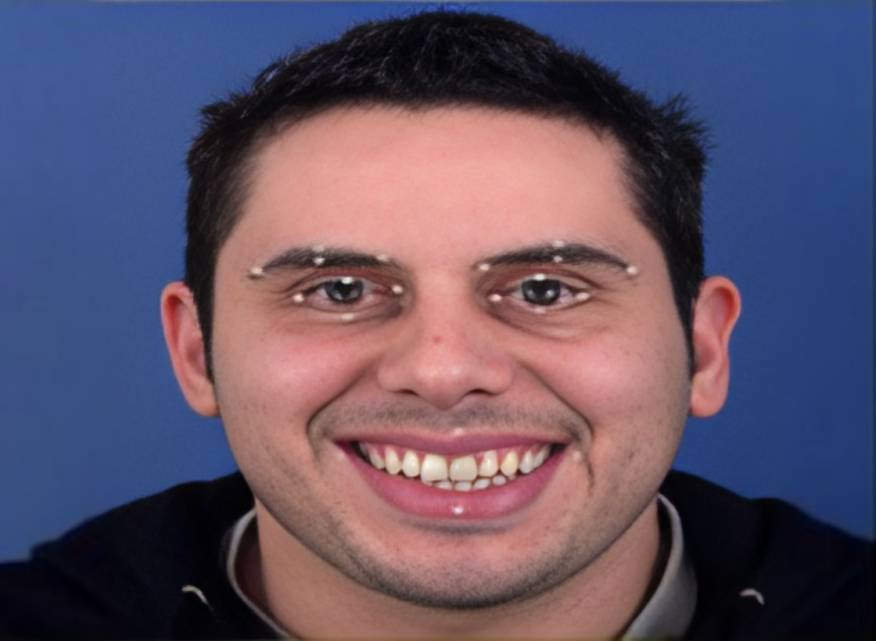
\includegraphics[scale=0.2]{gambar/2_2_1.png}
  % Keterangan gambar yang diinputkan
  \caption{\emph{Facial Landmarks} pada wajah objek}
  % Label referensi dari gambar yang diinputkan
  \label{fig:FacialLandmarks}
\end{figure}



\subsection{Deep learning}
\label{subsec:DeepLearning}

Deep learning merupakan cabang dari pembelajaran mesin yang 
menggunakan jaringan neural tiruan dengan banyak lapisan untuk 
memodelkan abstraksi data tingkat tinggi. Cara kerjanya 
melibatkan pemrosesan data melalui lapisan ini, dimana setiap 
lapisan secara otomatis dan secara progresif mempelajari 
fitur-fitur semakin kompleks dari data\parencite{akbulut2017deep}. Berbeda dengan 
pembelajaran mesin tradisional, deep learning dapat secara 
otomatis mengekstrak fitur penting tanpa memerlukan intervensi 
manual, memungkinkan model untuk melakukan tugas yang lebih 
kompleks dengan akurasi yang lebih tinggi. Keunggulan utama dari deep 
learning terletak pada kemampuannya untuk mengolah volume data 
yang sangat besar dan kompleks, memungkinkannya mengidentifikasi 
pola dan hubungan yang tidak dapat ditemukan oleh metode 
pembelajaran mesin konvensional. Hal ini membuat deep learning 
sangat efektif dalam aplikasi yang memerlukan analisis mendalam 
dari data visual, auditif, dan teks, memberikan dorongan 
signifikan dalam kemajuan teknologi pengenalan suara, visi 
komputer, dan pemrosesan bahasa alami.


\subsection{Percentage Of Eyelid Closure \emph{(PERCLOS)}}
PERCLOS atau biasa disebut Percentage of Eyelid Closure adalah salah 
satu metode yang digunakan untuk mendeteksi kantuk.
PERCLOS merupakan metrik yang digunakan untuk mengukur kantuk 
atau kelelahan pengemudi. Metode ini bekerja dengan cara 
menghitung persentase waktu dalam interval tertentu dimana dilakukan 
perhitungan bukaan kelopak mata seseorang tertutup sebagian atau 
seluruhnya di atas pupil. PERCLOS berfungsi sebagai indikator 
objektif untuk mengukur tingkat kantuk, berdasarkan frekuensi dan 
durasi penutupan mata meningkat seiring dengan kelelahan. 
PERCLOS efektif menunjukkan tingkat kelelahan pengemudi dan 
dianggap metode terbaik untuk mengukur kelelahan. Metode ini 
menghitung persentase waktu mata tertutup setidaknya 70 
atau 80 persen dari durasi total, yang umumnya adalah 30 
detik atau 1 menit. Guangyu,Jie,Licao melakukan penelitian dengan 
mengukur PERCLOS dan menghitung persentase frame dengan persentase mata tertutup 80 persen dalam video selama 30 detik 
dibagi dengan total frame selama 30 detik tersebut\parencite{Liu2023}. Atau dapat ditulis

\begin{equation}
  P80 = \frac{Frames with eyes closed to 80\% }{Total Frames of 30s video}
\end{equation}

(Liying,Haoxiang, 2008) menyatakan bahwa Tingkat pembukaan mata 
dapat dicirikan oleh bentuk pupil. Berdasarkan pengamatan bahwa 
saat mata tertutup, pupil mulai terhalang oleh kelopak mata dan 
bentuknya menjadi lebih elips. Oleh karena itu, mereka dapat 
menggunakan rasio sumbu elips pupil untuk menggambarkan tingkat 
pembukaan mata \parencite{lang2008study}. Untuk mendapatkan pengukuran yang lebih kuat 
untuk kedua parameter ini, dilakukan perhitungan rata-rata runtime 
(time tracking). Berdasarkan nilai rata-rata yang didapatkan, 
Liying,dkk dapat menganalisis keadaan waspada pengemudi. Mereka menghitung
2 parameter yang digunakan (rumus 2.1).

\begin{figure} [H] \centering
  % Nama dari file gambar yang diinputkan
  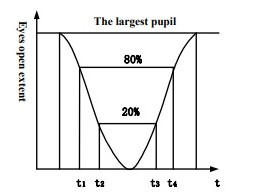
\includegraphics[scale=1]{gambar/2_2_2.jpg}
  % Keterangan gambar yang diinputkan
  \caption{Prinsip PERCLOS}
  % Label referensi dari gambar yang diinputkan
  \label{fig:PERCLOS}
\end{figure}

\subsection{Mouth Aspect Ratio (\emph{MAR})}
\label{subsec:MAR}

MAR atau Rasio Aspek Mulut adalah metrik analisis wajah yang 
digunakan untuk mendeteksi gerakan mulut yang berkaitan dengan 
berbagai kondisi, seperti berbicara, menguap, atau ekspresi emosi. 
Fungsinya adalah sebagai indikator kondisi ini dengan 
memperhitungkan kondisi geometris mulut seseorang pada waktu 
tertentu. Perhitungan MAR melibatkan analisis titik-titik 
tertentu di sekitar mulut dan menghitung rasio berdasarkan jarak 
antara titik-titik tersebut. Rasio ini kemudian dapat dipantau 
dari waktu ke waktu untuk mengamati perubahan yang mungkin sesuai 
dengan perilaku atau ekspresi tertentu. Pada deteksi kantuk,MAR (Mouth Aspect Ratio) dapat mengklasifikasikan kondisi kantuk pengemudi dengan mengukur perubahan geometri mulut berdasarkan titik-titik yang telah ditentukan pada model wajah. Titik-titik ini, yang mengelilingi bibir, digunakan untuk menghitung rasio yang mencerminkan pembukaan mulut. Ketika pengemudi mulai mengantuk, frekuensi dan durasi menguap meningkat, yang tercermin dalam nilai MAR yang lebih tinggi. Dengan memantau nilai ini, sistem dapat secara otomatis mendeteksi tanda-tanda awal kelelahan dan mengeluarkan peringatan kepada pengemudi.

\begin{figure} [H] \centering
  % Nama dari file gambar yang diinputkan
  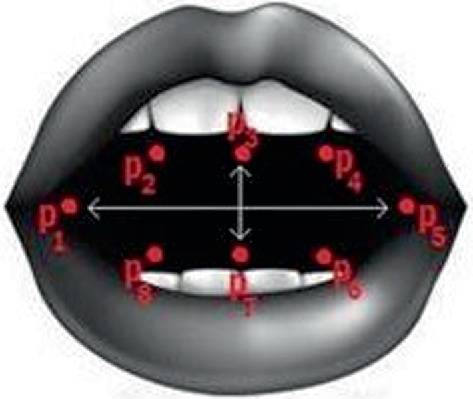
\includegraphics[scale=0.3]{gambar/2_2_3.png}
  % Keterangan gambar yang diinputkan
  \caption{MAR point}
  % Label referensi dari gambar yang diinputkan
  \label{fig:MAR}
\end{figure}


Pada gambar 2.3 terdapat sebanyak 8 titik yang saling berhubungan. titik-titik tersebut nantinya akan digunakan sebagai acuan agar dilakukan perhitungan. Hasil perhitungan ini disebut sebagai hasil lokalisasi kemudian menghasilkan nilai MAR. Nilai MAR dapat ditentukan dengan rumus sebagai berikut. Dimana |p2-p8| adalah nilai hasil perhitungan Jarak Euclidean antara koordinat titik-titik fitur pada wajah, dan delapan titik fitur kunci yang berkorespondensi dengan variabel dalam rumus sebagaimana ditampilkan pada gambar 2.3. Jarak Euclidean ini dihitung dengan mengambil akar kuadrat dari perbedaan kuadrat koordinat horizontal dan vertikal dari dua titik fitur tersebut\parencite{chandiwala2021driver}.

\begin{equation}
MAR = \frac{|{p2} - {p8}| + |{p3} - {p7}| + |{p4} - {p6}|}{3|{p1} - {p5}|}
\end{equation}


\subsection{Skala Kantuk Karolinska}
\label{subsec:KSS}
\newcommand{\w}{}
\newcommand{\G}{\cellcolor{gray}}
\begin{table}[h!]
  \centering
  \caption{Skala Kantuk Karolinska}
  \begin{tabular}{|c|l|}
    \hline
    Skala \G & Penjelasan \G  \\
    \hline
    1 & Amat sangat terjaga \\
    2 & Sangat terjaga \\
    3 & Terjaga \\
    4 & Cukup terjaga \\
    5 & Antara terjaga dan mengantuk \\
    6 & Muncul mengantuk \\
    7 & Mengantuk namun tidak sulit untuk terjaga/kantuk ringan \\
    8 & Sangat mengantuk, sulit terjaga \\
    9 & Amat sangat mengantuk, cenderung tidak sadar \\
    \hline
  \end{tabular}
  \label{tab:SkalaKSS}
\end{table}


Skala Kantuk Karolinska, yang dikenal juga dengan Karolinska Sleepiness Scale (KSS), adalah skala yang digunakan untuk mengukur kantuk secara subjektif. Skala ini berkisar dari 1 hingga 9, dengan 1 mengindikasikan tingkat kesegaran tinggi dan 9 menunjukkan kesulitan yang sangat besar untuk tetap terjaga. Skala Kantuk Karolinska (KSS) dapat digunakan sebagai alat pengklasifikasi kantuk dengan beberapa cara. Pada beberapa penelitian yang telah dilakukan, KSS digunakan sebagai pengklasifikasi kantuk. Dengan metode skala kantuk karolinska,terlihat bahwa klasifikasi kantuk yang dilakukan memiliki hasil akurasi yang tinggi dimana artinya KSS terbukti valid dijadikan sebagai acuan skala klasifikasi kantuk.

\subsection{Support Vector Machine \emph{(SVM)}}
\label{subsec:SVM}

Dalam lingkup Deep learning atau tepatnya supervised learning, Support Vector Machine (SVM) merupakan metode klasifikasi dan regresi yang efektif. SVM beroperasi dengan mengembangkan konsep hyperplane yang optimal, yang secara matematis didefinisikan sebagai batas pemisah yang paling efisien antara kelas-kelas data. Algoritma ini melibatkan identifikasi margin terlebar yang memungkinkan pemisahan kelas dengan paling jelas, yang bertujuan untuk meningkatkan akurasi prediksi model pada data baru. Dalam ruang dua dimensi, hyperplane ini dapat berupa garis lurus, tetapi dalam ruang tiga dimensi atau lebih, ia menjadi bidang pemisahan multidimensi. Kemampuan SVM untuk mengadaptasi diri dengan masalah linear dan non-linear menjadikannya pilihan yang kuat dalam berbagai aplikasi pembelajaran mesin, dari pengenalan gambar hingga pemodelan prediktif dalam keuangan.  

\begin{figure} [H] \centering
  % Nama dari file gambar yang diinputkan
  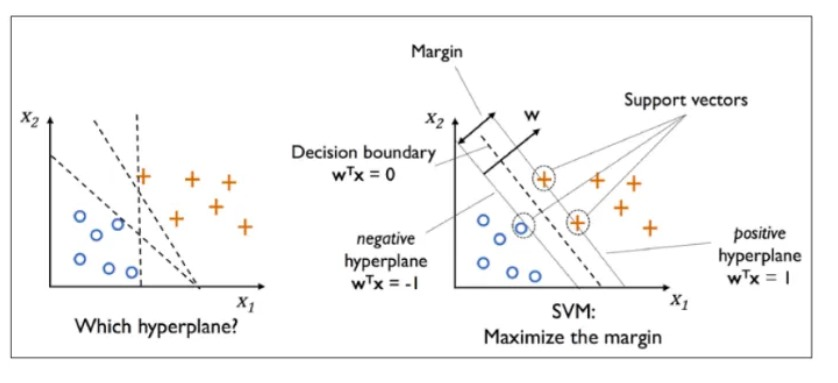
\includegraphics[scale=0.7]{gambar/2_2_6.jpg}
  % Keterangan gambar yang diinputkan
  \caption{Hyperplane yang memisahkan kelas positif dan negatif}
  % Label referensi dari gambar yang diinputkan
  \label{fig:SVM}
\end{figure}

Pada gambar 2.4, dapat dilihat bahwa ada perbedaan jarak antara hyperplane dengan kedua kelas baik itu kelas positif atau negatif dimana pada gambar tersebut kelas negatif bertanda bulat. Dengan SVM, objek terdekat dengan hyperplane dikenali dengan nama Support Vector. Objek tersebut baik itu dari kelas negatif atau positif dapat dikatakan sulit untuk diklasifikasikan. Hal tersebut terjadi karena data kelas tersebut sangat berdekatan dengan data kelas lain sehingga menyebabkan hampir terjadinya overleap\parencite{tan2018research}. Oleh karena itu,dengan menggunakan SVM,kondisi ini dapat dimimalisir dimana hasil dari perhitungan akan memisahkan dan menentukan kelas dari data yang terkena overleap tersebut.


\subsection{SMOTE}
\label{subsec:SMOTE}
SMOTE (Synthetic Minority Over-sampling Technique) adalah metode yang digunakan dalam pengolahan data untuk mengatasi masalah ketidakseimbangan kelas. Teknik ini menghasilkan sampel data sintetis untuk kelas minoritas dengan cara interpolasi antara sampel minoritas yang ada. Hal ini membantu dalam memperbaiki keseimbangan antara kelas minoritas dan mayoritas, dimana hal tersebut merupakan hal yang penting dalam model pembelajaran mesin untuk meningkatkan kinerja dan hasil yang lebih akurat dalam prediksi.


\begin{figure} [H] \centering
  % Nama dari file gambar yang diinputkan
  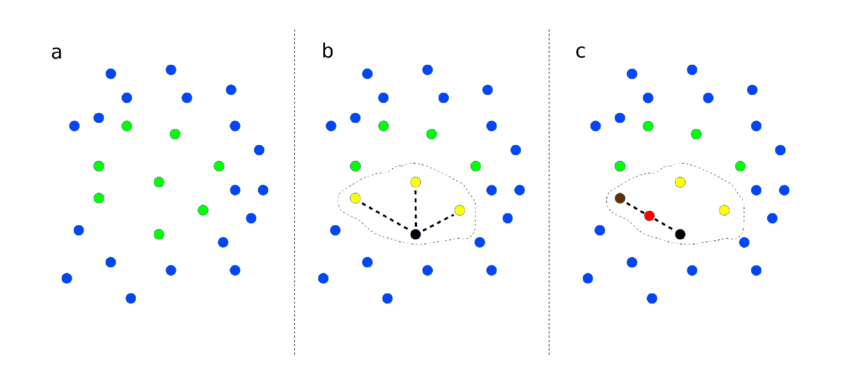
\includegraphics[scale=0.5]{gambar/2_2_5.png}
  % Keterangan gambar yang diinputkan
  \caption{Ilustrasi Visual SMOTE}
  % Label referensi dari gambar yang diinputkan
  \label{fig:SMOTE}
\end{figure}

Gambar 2.4 Merepresentasikan grafis algoritma SMOTE,dimulai dengan sample set positif (titik berwarna hijau),dan sample set negatif (titik berwarna biru). Algoritma ini kemudian memilih sebuah sample positif (titik berwarna hitam) dan kNN diantara titik positif (dengan warna kuning dengan k=3), kemudian akhirnya,salah satu dari kNN secara acak terpilih yang mana kemudian titik positif sintetis baru tercipta dengan secara acak menghasilkan sebuah model baru sepanjang garis lurus yang terhubung dengan titik hitam dan coklat\parencite{schubach2017imbalance}.

\cleardoublepage

% Bab 3 desain dan implementasi
\chapter{DESAIN DAN IMPLEMENTASI}
\label{chap:desainimplementasi}

% Ubah bagian-bagian berikut dengan isi dari desain dan implementasi

Pada bab ini akan dijelaskan mengenai bagaimana cara sistem bekerja sehingga menghasilkan output yang diinginkan. Sistem dibuat bertujuan untuk membuat model klasifikasi menggunakan support vertor machine sebagai alat yang akan mempelajari data input dan membuat model klasifikasi tingkat kantuk dengan menggunakan parameter PERCLOS dan MAR.

\section{Metode yang digunakan}
\label{sec:Metode} 


% Contoh input gambar dengan format *.jpg
\begin{figure} [H] \centering
  % Nama dari file gambar yang diinputkan
  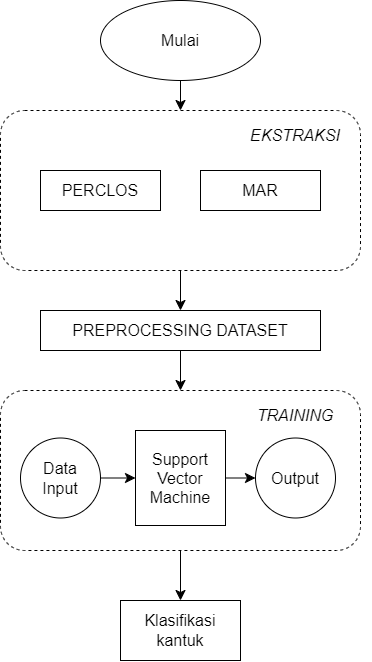
\includegraphics[scale=0.45]{gambar/2_2_7.png}
  % Keterangan gambar yang diinputkan
  \caption{Diagram Alur model}
  % Label referensi dari gambar yang diinputkan
  \label{fig:Diagram}
\end{figure}

% Contoh penggunaan referensi dari gambar yang diinputkan
Pada \emph{Diagram} yang tertera di Gambar \ref{fig:Diagram}. Akan digunakan metode seperti berikut :

\subsection{Pengumpulan Dataset}

Dalam penggunaan dataset,diperlukan beberapa kriteria sebagai input data yang kemudian nantinya akan diolah. Pada penelitian kali ini, akan digunakan dataset yang telah terverifikasi yaitu UTA-RLDD dataset. Data yang digunakan mempunyai durasi yang cukup untuk digunakan sebagai dataset. Kemudian dataset UTA-RLDD memiliki berbagai objek yang berbeda baik itu dari wajah, jenis kelamin, atau etnis. Data yang digunakan merupakan video yang memiliki fps rata-rata sekitar 30 FPS. Dataset UTA-RLDD akan digunakan untuk data testing dari model yang akan dibuat. Kemudian selain itu digunakan juga dataset DROZY. Dataset ini nantinya akan dilakukan ekstraksi nilai PERCLOS dan MAR dan kemudian diolah sehingga menghasilkan model yang diinginkan. 


\begin{figure} [H] \centering
  % Nama dari file gambar yang diinputkan
  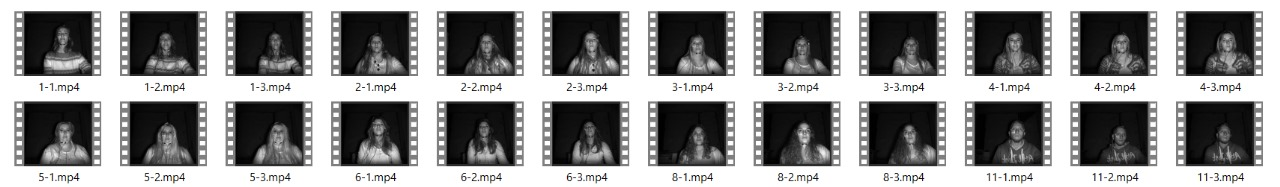
\includegraphics[scale=0.4]{gambar/3_1_4.jpg}
  % Keterangan gambar yang diinputkan
  \caption{Kumpulan Dataset}
  % Label referensi dari gambar yang diinputkan
  \label{fig:DatasetPic}
\end{figure}

\subsection{Preprocessing Dataset}
\label{subsec:Preprocessing}
\begin{enumerate}
  \item{\textbf{Interpolasi Frame Dataset}}
  
  Interpolasi frame Dataset dalam penelitian ini adalah video, merupakan teknik yang digunakan untuk meningkatkan jumlah frame per detik (FPS) dari sebuah video, sehingga menghasilkan pemutaran yang lebih halus. Salah satu metode yang umum digunakan untuk interpolasi frame video adalah melalui penggunaan encoder. Encoder bekerja dengan menambahkan frame baru antara frame asli video, menggunakan algoritma interpolasi untuk memperkirakan posisi objek dan piksel di antara frame asli tersebut. Hal ini sering dilakukan dengan bantuan perangkat keras khusus atau software yang mendukung pemrosesan video secara efisien.

  \begin{figure} [H] \centering
    % Nama dari file gambar yang diinputkan
    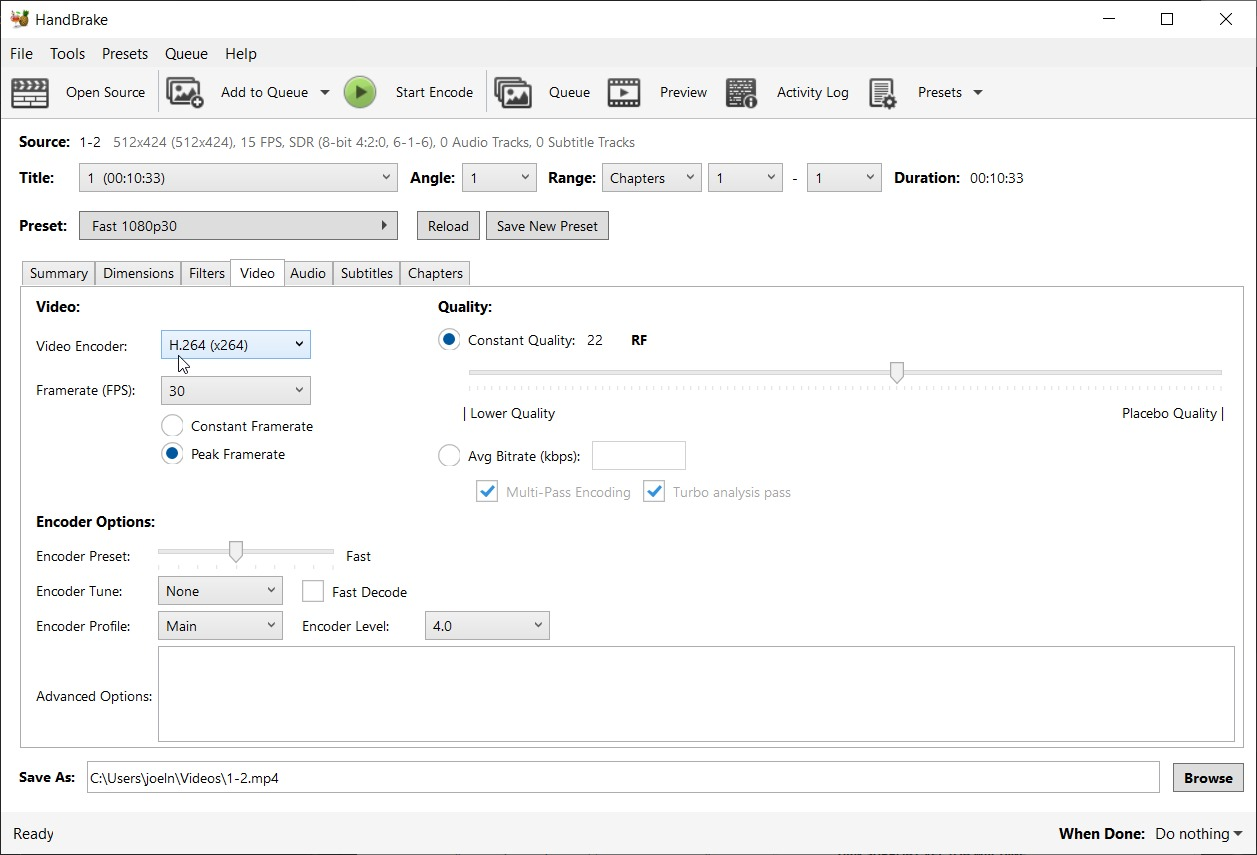
\includegraphics[scale=0.2]{gambar/Handbrake.jpg}
    % Keterangan gambar yang diinputkan
    \caption{HandBrake}
    % Label referensi dari gambar yang diinputkan
    \label{fig:HandBrake}
  \end{figure}

Salah satu software populer yang dapat digunakan untuk interpolasi frame video adalah HandBrake. HandBrake adalah alat open-source yang kuat untuk mengonversi dan memproses video, termasuk kemampuan untuk mengubah frame rate video. Dengan HandBrake, pengguna dapat meningkatkan FPS video dengan cara mengonfigurasi pengaturan encoding. Dalam proses ini, HandBrake menggunakan teknik interpolasi frame untuk menambahkan frame tambahan, menghasilkan video dengan frame rate yang lebih tinggi dan pemutaran yang lebih mulus. Prosesnya dimulai dengan membuka file video dalam HandBrake dan memilih preset yang sesuai atau mengonfigurasi pengaturan secara manual. Pengguna dapat mengatur frame rate target yang diinginkan, misalnya dari 15 FPS menjadi 30 FPS. HandBrake kemudian menggunakan encoder untuk melakukan interpolasi, menambahkan frame baru di antara frame yang sudah ada berdasarkan algoritma interpolasi yang dipilih. Setelah pengaturan selesai, proses encoding dimulai, dan HandBrake menghasilkan file video baru dengan frame rate yang lebih tinggi.

\begin{figure}[htbp]
  \centering
  \subfigure[FPS sebelum Interpolasi]{
    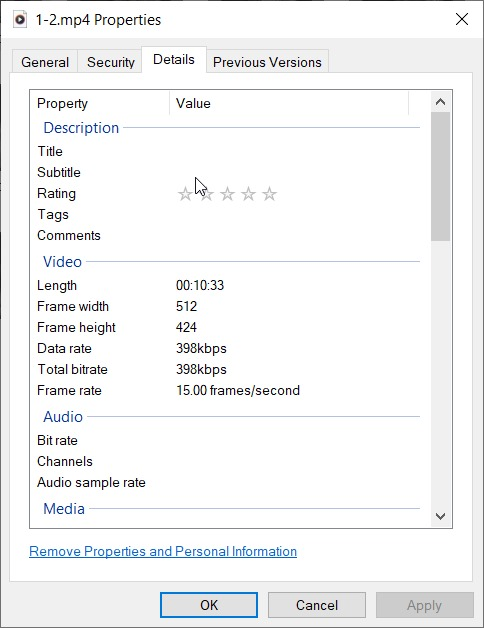
\includegraphics[scale=0.5]{gambar/Hasil1.jpg}
    \label{fig:FPS}
  }
  \hspace{0.5cm}
  \subfigure[FPS sesudah Interpolasi]{
    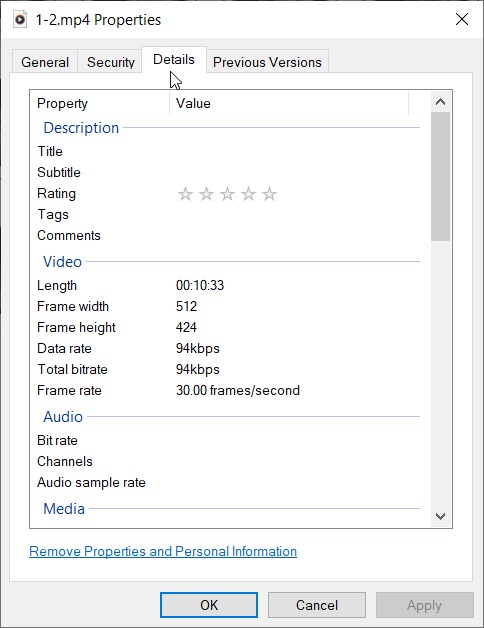
\includegraphics[scale=0.5]{gambar/hasil2.jpg}
    \label{fig:FPS2}
  }
  \caption{Perbandingan FPS sebelum dan sesudah interpolasi}
  \label{fig:FPS_comparison}
\end{figure}

  \item {\textbf{Landmark Dataset}}
  
  Pada proses deteksi fitur wajah dalam video yang dilakukan dengan PyCharm dan library Dlib, digunakan pendekatan deteksi landmark wajah melalui Histogram of Oriented Gradients (HOG) dan Support Vector Machine (SVM). Metode ini memberikan hasil identifikasi wajah yang akurat dalam video. Proses dimulai dengan deteksi wajah menggunakan HOG, yang merupakan teknik ekstraksi fitur yang kuat dalam mengenali wajah dengan berbagai orientasi dan kondisi pencahayaan. HOG bekerja dengan menghitung orientasi gradien di area gambar dan membuat histogram untuk mewakili distribusi gradien tersebut. Selanjutnya, SVM digunakan untuk mengklasifikasikan area yang mengandung wajah berdasarkan fitur HOG yang diekstraksi. SVM sangat efektif dalam membedakan antara wajah dan non-wajah karena kemampuannya untuk menemukan hyperplane optimal yang memisahkan dua kelas.

Setelah wajah terdeteksi, prediktor landmark dari Dlib digunakan untuk mengenali dan memetakan titik-titik penting pada wajah. Dlib menyediakan model pra-terlatih yang dapat mengenali 68 titik landmark pada wajah, mencakup area seperti mata, alis, hidung, mulut, dan kontur wajah. Proses ini melibatkan regresi ensemble yang memprediksi lokasi landmark berdasarkan citra input, memberikan koordinat yang presisi untuk setiap titik landmark. Dengan menggunakan 68 titik landmark ini, kita dapat melakukan berbagai analisis wajah lebih lanjut. Contohnya, koordinat dari landmark mata digunakan untuk menghitung Eye Aspect Ratio (EAR), yang merupakan indikator untuk mendeteksi kondisi mata tertutup atau terbuka. Selain itu, koordinat dari landmark mulut digunakan untuk menghitung Mouth Aspect Ratio (MAR), yang mengukur lebar dan tinggi mulut untuk mendeteksi ekspresi wajah seperti senyum atau menguap.

\begin{figure} [H] \centering
  % Nama dari file gambar yang diinputkan
  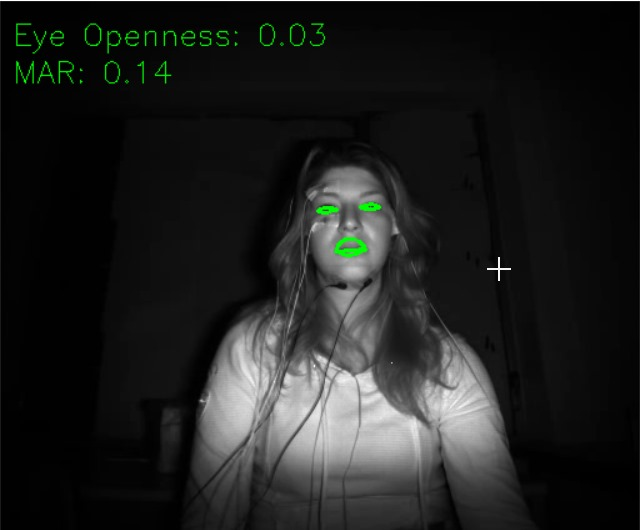
\includegraphics[scale=0.5]{gambar/3_1_2.jpg}
  % Keterangan gambar yang diinputkan
  \caption{Landmark Wajah}
  % Label referensi dari gambar yang diinputkan
  \label{fig:LandmarkW}
\end{figure}


  \item {\textbf{Ekstraksi Bukaan Mata dan Mulut}}
  
  \textbf{a. Deteksi Mata Kanan dan Mata Kiri}

  Setelah wajah terdeteksi, model prediktor landmark dari Dlib digunakan untuk mengenali dan memetakan titik-titik penting pada wajah. Dlib menyediakan model yang dapat mengenali 68 titik landmark pada wajah, mencakup area seperti mata, alis, hidung, mulut, dan kontur wajah. Dalam konteks ekstraksi mata, titik-titik landmark yang relevan adalah Mata Kiri: Titik 36 hingga 41. Mata Kanan: Titik 42 hingga 47.

Titik-titik ini memetakan kontur mata secara akurat. Untuk visualisasi, mata kiri biasanya digambarkan dengan warna hijau, sedangkan mata kanan digambarkan dengan warna merah, seperti yang terlihat pada gambar. Warna-warna ini membantu dalam membedakan antara mata kiri dan kanan dengan jelas. Proses selanjutnya melibatkan penggunaan koordinat dari titik-titik landmark tersebut untuk menggambar kontur di sekitar mata. Kontur ini digambar menggunakan fungsi dari OpenCV yang memungkinkan visualisasi yang jelas dari area mata.

\begin{figure} [H] \centering
  % Nama dari file gambar yang diinputkan
  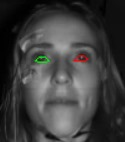
\includegraphics[scale=1.65]{gambar/mata.jpg}
  % Keterangan gambar yang diinputkan
  \caption{Landmark mata}
  % Label referensi dari gambar yang diinputkan
  \label{fig:Landmarkmata}
\end{figure}

  \textbf{b. Hitung Luasan Mata dan Mulut}

  Gambar 3.6 menunjukkan area yang ditandai hanya pada mata. Hal ini dilakukan sehingga hanya area mata yang dibutuhkan pada wajah untuk penelitian ini. Selanjutnya, area mata ini yang difokuskan, sehingga melalui koordinat yang ada, mata kanan dan mata kiri dapat dipisah atau dipotong. Setelah dipotong, setiap mata dibuat menjadi citra binary, sehingga hanya tersisa warna hitam dan putih. Gambar 3.7 menunjukkan mata yang telah dipotong dan dibuat ke binary.

  \begin{figure}[htbp]
    \centering
    \subfigure[left Eye]{
      
\includegraphics[scale=5]{gambar/lefteye.jpg}
      \label{fig:left}
    }
    \hspace{0.5cm}
    \subfigure[Right Eye]{
      
\includegraphics[scale=5]{gambar/righteye.jpg}
      \label{fig:right}
    }
    \caption{Binary Eye}
    \label{fig:Binary_eye}
  \end{figure}
  

Mata yang dibuat ke binary ini dilakukan masking agar area yang berwarna hitam hanya pada mata dan sekitarnya berwarna putih. Gambar 3.7 menunjukkan hanya mata saja yang berwarna putih. Hal ini dibutuhkan untuk dilanjutkan ke tahap berikutnya, yaitu mencari luas berdasarkan piksel berwarna putih. Setelah sampai pada tahap masking mata, seperti pada Gambar 3.7, maka tahap selanjutnya adalah mendapatkan luas mata. Luas mata dapat dihitung dengan menjumlahkan semua piksel yang berwarna putih. Berdasarkan hal ini, maka apabila mata seseorang terbuka, maka area berwarna putih juga akan meluas, sebaliknya, apabila mata seseorang tertutup, maka luas mata yang berwarna putih akan mengecil.

Perhitungan nilai Openness dilakukan dengan membandingkan jumlah piksel berwarna putih pada citra mata binary terhadap total piksel pada citra tersebut. Nilai Openness memberikan indikasi seberapa terbuka mata seseorang dalam frame tersebut. Sedangkan, Mouth Aspect Ratio (MAR) dihitung menggunakan koordinat dari titik-titik landmark pada mulut, dengan rumus yang memperhitungkan jarak antara titik-titik tertentu di bagian atas dan bawah serta sisi-sisi mulut. MAR memberikan indikasi tentang ekspresi wajah, seperti menguap atau berbicara.

\begin{figure} [H] \centering
  % Nama dari file gambar yang diinputkan
  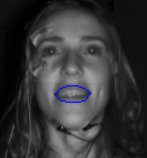
\includegraphics[scale=1.65]{gambar/mouth.jpg}
  % Keterangan gambar yang diinputkan
  \caption{Landmark mulut}
  % Label referensi dari gambar yang diinputkan
  \label{fig:Landmarkmulut}
\end{figure}

  \textbf{c. Interpolasi Data Luas Mata dan Mulut}

Pada proses ini, dilakukan optimasi pada hasi data yang didapatkan. Karena saat pemrosesan video, ada frame-frame yang tidak terdeteksi landmark-nya sehingga membuat data Openness dan MAR menjadi 0, diperlukan optimasi agar data yang hilang tersebut dapat direkonstruksi secara sintetis. Optimasi atau rekonstruksi ini dilakukan dengan menggunakan metode interpolasi. Pada penelitian ini digunakan interpolasi linear, di mana data yang diinterpolasi adalah hasil ekstraksi nilai Openness dan MAR.

Interpolasi linear adalah metode yang sederhana dan efektif untuk memperkirakan nilai-nilai di antara dua titik data yang diketahui. Dalam konteks ini, jika data Openness dan MAR pada frame tertentu tidak terdeteksi (bernilai 0), nilai tersebut diganti menjadi NaN (Not a Number). Kemudian, interpolasi linear digunakan untuk mengisi nilai-nilai NaN tersebut. Proses interpolasi linear bekerja dengan menggambar garis lurus antara dua titik data yang diketahui dan menggunakan garis tersebut untuk memperkirakan nilai di antara kedua titik. Dengan menggunakan interpolasi linear, nilai-nilai Openness dan MAR yang hilang dapat diisi dengan nilai yang logis dan konsisten dengan perubahan asli, menghasilkan transisi yang halus antara nilai tiap frame dan meningkatkan fluiditas hasil analisis video. Teknik ini membantu mengatasi masalah data yang hilang akibat deteksi landmark yang tidak sempurna, memastikan bahwa analisis tetap akurat dan andal.
\end{enumerate}

\subsection{Hitung data PERCLOS dan MAR}
\label{subsec:HitungPERCLOS}
 Berdasarkan penelitian \parencite{7545182}. Untuk mendapatkan nilai PERCLOS, pertama sekali diperlukan nilai treshold untuk menentukan nilai acuan untuk menentukan apakah kondisi mata sedang terbuka atau tertutup. Untuk mencari treshold ditentukan diurutkan data mulai dari tertinggi sampai pada data yang bernilai terendah. Pengurutan data ini dilakukan kepada tiap data atau file csv yang berisi nilai bukaan mata sebelumnya. Sehingga, nilai treshold yang dimiliki tiap data atau tiap file csv memiliki nilai yang berbeda.

 Setelah data diurutkan, kemudian dilakukan perhitungan rata rata untuk mendapatkan nilai rata rata O dan C. Untuk mendapatkan nilai O, dilakukan perhitungan 1/20 total data. Hasil dari nilai 1/20 total data ini digunakan untuk mengambil data teratas sebanyak hasil 1/20 total data sebelumnya dan kemudian dirata ratakan untuk mendapatkan nilai O. Sebaliknya, dari data paling rendah diambil sebanyak 1/20 total data dan kemudian dirata ratakan untuk mendapatkan nilai C. Setelah itu dilakukan perhitungan treshold dengan menggunakan rumus 3.1.

 \begin{equation}
  Threshold = (O - C)* 0,2 + C
\end{equation}


Kemudian setelah didapatkan nilai treshold nya, semua data yang berada di atas treshold dikelompokkan per 30 frame data. Sehingga total nilai nya dianggap sebagai nIO, sedangkan data yang bernilai dibawah treshold dikelompokkan per 30 frame data,dijumlahkan dan dianggap sebagai nIC. Setelah masing masing nilai didapat, maka nilai PERCLOS bisa didapat. Untuk rumus PERCLOS dapat dilihat pada rumus 3.2. 

\begin{equation}
\label{eq:PERCLOSeq}
  PERCLOS = \frac{\emph{nIC} }{\emph{nIC} + \emph{nIO}}
\end{equation}

Perhitungan ini dilakukan terhadap semua file csv yang berisi data bukaan mata. Sehingga total data PERCLOS yang didapatkan berbeda pula.

Sedangkan untuk perhitungan nilai MAR, digunakan rumus 2.2. Titik-titik landmark diperoleh dari model prediktor landmark wajah, seperti yang disediakan oleh Dlib. Penghitungan jarak Euclidean antara titik-titik ini memberikan ukuran yang digunakan untuk menghitung MAR. Dengan kata lain, MAR adalah perbandingan antara lebar vertikal dan horizontal mulut, memberikan indikator yang dapat digunakan untuk analisis ekspresi wajah. Nilai MAR yang tinggi menunjukkan bahwa mulut lebih terbuka, yang bisa mengindikasikan menguap atau berbicara, sedangkan nilai yang lebih rendah menunjukkan mulut yang lebih tertutup. 

\begin{lstlisting}[
  language=Python,
  caption={Menghitung PERCLOS.},
  label={lst:PERCLOS}
]
import pandas as pd

def calculate_threshold(chunk):
    """
    Hitung threshold untuk chunk data.
    """
    total_frames = len(chunk)
    A = total_frames // 20
    A = max(A, 1)

    sorted_data = chunk.sort_values(by='EAR', ascending=False)

    O = sorted_data['EAR'].head(A).mean()
    C = sorted_data['EAR'].tail(A).mean()

    threshold = (O - C) * 0.2 + C

    return threshold

def process_data(file_path):
    df = pd.read_csv(file_path)
    if 'EAR' not in df.columns or 'MAR' not in df.columns:
        raise ValueError("Kolom 'EAR' atau 'MAR' tidak ditemukan dalam file CSV")
    
    result = []

    for i in range(0, len(df), 30):
        chunk = df.iloc[i:i+30]
        
        if len(chunk) == 0:
            continue
        
        threshold = calculate_threshold(chunk)

        chunk_openness = chunk['EAR']
        chunk_mar = chunk['MAR']

        above_threshold = chunk_openness[chunk_openness > threshold]
        below_threshold = chunk_openness[chunk_openness <= threshold]
        
        sum_above = above_threshold.sum()
        sum_below = below_threshold.sum()

        std_mar = chunk_mar.std()
        
        result.append({
            'Sum_Above_Threshold': sum_above,
            'Sum_Below_Threshold': sum_below,
            'MAR_Std': std_mar
        })

    result_df = pd.DataFrame(result)
    
    return result_df

def calculate_ratio(data):
    data['PERCLOS'] = data['Sum_Below_Threshold'] / (data['Sum_Above_Threshold'] + data['Sum_Below_Threshold'])
    
    result_df = data[(data['PERCLOS'] > 0) & (data['PERCLOS'] < 0.8)]
    result_df = result_df[['PERCLOS', 'MAR_Std']]
    
    return result_df

file_path = r'F:\SKRIPSI\TA\Fix_code\SkripSHYs\DataEARMAR\14-3_data_analysis.csv'
final_output_path = r'F:\SKRIPSI\TA\Fix_code\SkripSHYs\PERCLOS\Perclos\14-3_final_result.csv'

processed_data = process_data(file_path)
final_result = calculate_ratio(processed_data)
final_result.to_csv(final_output_path, index=False)

print(f"Proses selesai. Hasil disimpan di {final_output_path}")


\end{lstlisting}




\subsection{Labeling Data}
\label{subsec:Labelling}

Dalam tahapan preprocessing, proses labeling merupakan langkah krusial setelah interpolasi frame. Labeling melibatkan pengkategorian data berdasarkan karakteristik tertentu untuk memudahkan proses training. Sebelum data di training tentunya data harus diberikan label agar nantinya data tersebut dapat dikenali dan dipelajari oleh machine learning. Proses ini bertujuan untuk menandai frame-frame dalam dataset video dengan label yang menunjukkan informasi tertentu, seperti tingkat keaktifan, ekspresi wajah, atau indikator kantuk pada subjek yang diamati. Dalam penelitian ini, labeling digunakan untuk memberikan informasi kelas kantuk yang dimiliki oleh data yang kita akan gunakan. Keakuratan dalam labeling secara langsung mempengaruhi kualitas hasil analisis menggunakan model pembelajaran mesin. Kesalahan dalam labeling dapat mengarah pada pembelajaran yang salah oleh model, yang pada akhirnya menurunkan performa model saat digunakan dalam pengujian nyata atau implementasi.

\begin{figure} [H] \centering
  % Nama dari file gambar yang diinputkan
  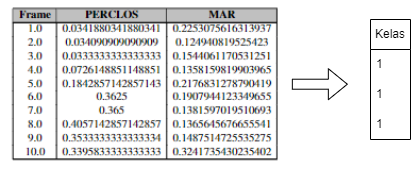
\includegraphics[scale=0.75]{gambar/label.png}
  % Keterangan gambar yang diinputkan
  \caption{Labelling }
  % Label referensi dari gambar yang diinputkan
  \label{fig:labell}
\end{figure}


\subsection{Balancing Data}
\label{subsec:Balancing}

Pada bagian ini akan dilakukan penyeimbangan data. Balancing data, atau penyeimbangan data, merupakan proses mengatasi permasalahan imbalance dalam dataset, yaitu ketika jumlah sampel untuk setiap kelas dalam data tidak seimbang. Fungsi balancing data adalah untuk meningkatkan kinerja model dengan memastikan bahwa setiap kelas diwakili secara adil dalam proses training
Dengan memastikan bahwa data untuk setiap kelas seimbang, model dapat belajar fitur dari setiap kelas secara lebih efektif, yang pada gilirannya dapat meningkatkan akurasi dan kinerja model secara keseluruhan.

Beberapa metode populer untuk balancing data meliputi:

Oversampling: Meningkatkan jumlah sampel dalam kelas minoritas dengan cara membuat duplikat sampel yang ada atau menambahkan sampel sintetis (misalnya, menggunakan teknik SMOTE - Synthetic Minority Over-sampling Technique).

Undersampling: Mengurangi jumlah sampel dalam kelas mayoritas untuk mencocokkan jumlah sampel di kelas minoritas. Metode ini bisa mengurangi informasi karena menghilangkan sampel dari dataset.

Pada tahap ini, diterapkan metode SMOTE (Synthetic Minority Over-sampling Technique) untuk penyeimbangan data.  Neighbors (KNN) untuk memilih sampel minoritas terdekat, kemudian menciptakan sampel baru di sepanjang garis yang menghubungkan sampel minoritas yang dipilih. Dengan cara ini, SMOTE dapat meningkatkan jumlah sampel dalam kelas minoritas secara lebih efektif dan realistis, sehingga membantu model belajar fitur dari kelas minoritas dengan lebih baik. Penerapan SMOTE dalam tahap ini membantu memastikan bahwa dataset yang digunakan untuk training model memiliki representasi yang seimbang dari setiap kelas. Hal ini sangat penting dalam situasi di mana ada perbedaan besar antara jumlah sampel kelas mayoritas dan minoritas, yang jika tidak ditangani, dapat menyebabkan model menjadi bias dan kurang akurat dalam memprediksi kelas minoritas.

\subsection{Data Model}
\label{subsec:datamodel}

Setelah dilakukan balancing data, didapatkan jumlah data yang diharapkan siap untuk dilakukan training. Setelah balancing dilakukan, bentuk dari data yang akan ditraining juga disesuaikan agar dapat dibaca dengan baik oleh kernel yang akan digunakan untuk melatih data. Pada tabel

% Please add the following required packages to your document preamble:
% \usepackage{booktabs}
% \usepackage[table,xcdraw]{xcolor}
% Beamer presentation requires \usepackage{colortbl} instead of \usepackage[table,xcdraw]{xcolor}
\begin{table}[]
  \resizebox{\textwidth}{!}{%
    \begin{tabular}{@{}|l|l|l|@{}}
      \toprule
      \rowcolor[HTML]{9B9B9B} 
      \textbf{PERCLOS}                                                                              & \textbf{MAR\_Std}                                                                             & \textbf{Class} \\ \midrule
      {[}0.04341892752775, 0.0457977178822792, 0.0363179516630053, ..... ,0.0244741972028755{]}     & {[}0.0246262117542063, 0.0286218820410614, 0.0193095358670792, ..... , 0.0261656150259289{]}  & 1              \\ \midrule
      {[}0.0400738453832094, 0.0972990335686605, 0.0547994224962394, ..... ,0.069500642000451{]}    & {[}0.0141064884833305, 0.0204998221406212, 0.014796507161195, ..... , 0.0151702160660887{]}   & 2              \\ \midrule
      {[}0.0412412516391, 0.036259197114398, 0.0502209552341277, ..... , 0.1099072500438651{]}      & {[}0.0200517953558288, 0.0171611029328477, 0.0226213027135124, ..... , 0.0170603553394825{]}  & 3              \\ \midrule
      {[}0.0213255394874295, 0.0833854160470106, 0.1656879279840406, ..... , 0.2286525334203849{]}  & {[}0.020227686316819, 0.0243025111247356, 0.0154098099944, ..... , 0.0186653390589496{]}      & 1              \\ \midrule
      {[}0.0636015655556773, 0.0395954952422416, 0.0635752407017011, ..... , 0.1003420550712484{]}  & {[}0.0208416492197107, 0.0138630902415231, 0.014491989523608, ..... , 0.0176932533766617{]}   & 3              \\ \midrule
      {[}0.0842387212944913, 0.045642823859335, 0.0409224457104011, ..... , 0.0255765930580907{]}   & {[}0.0140002122149792, 0.0157727917200389, 0.0153864082286545, ..... , 0.0151854902506547{]}  & 3              \\ \midrule
      {[}0.1414414688557654, 0.0750010180340961, 0.0483832632916631, ..... , 0.0242062194483447{]}  & {[}0.0176113769338634, 0.0127499041911238, 0.0161585952725352, ..... , 0.0139200535625622{]}  & 2              \\ \midrule
      {[}0.0234181791077069, 0.020206567887021, 0.0224715053110436, ..... , 0.2141770174091717{]}   & {[}0.0200319424575923, 0.0152445913516931, 0.0111976782111738, ..... , 0.0140688048915294{]}  & 3              \\ \midrule
      {[}0.0498987673077989, 0.0420765550820641, 0.0729490921842854, ..... , 0.0375348918417948{]}  & {[}0.0150412651906854, 0.0144975684090787, 0.0207710633109784, ..... , 0.0166353062050138{]}  & 1              \\ \midrule
      {[}0.0174667811334755, 0.0524654907429773, 0.1146293828800185, ..... , 0.0665150468025401{]}  & {[}0.0333034331494606, 0.0295097688107696, 0.0179873633974712, ..... , 0.0139688372216801{]}  & 1              \\ \midrule
      {[}0.0372463645779023, 0.0768757764497994, 0.0694498634569315, ..... , 0.1775682670898423{]}  & {[}0.0168976539192993, 0.0177318180221479, 0.0132788222345029, ..... , 0.0180524048238422{]}  & 2              \\ \midrule
      {[}0.0225255789092395, 0.1589413770035415, 0.0228244609011684, ..... , 0.0973160030637269{]}  & {[}0.0144051993419015, 0.0145949179613355, 0.0111113433985775, ..... , 0.0138968269424785{]}  & 3              \\ \midrule
      {[}0.0909425380749068, 0.02538180602124, 0.0262281644443559, ..... , 0.0276037323400727{]}    & {[}0.0113076467960533, 0.010084838884392, 0.0096172036699211, ..... , 0.015381471540111{]}    & 2              \\ \midrule
      {[}0.0697078436865611, 0.0220805884255913, 0.0231435028540088, ..... , 0.5867753807455728{]}  & {[}0.0169111714521571, 0.0160535663464046, 0.0203783646065001, ..... , 0.0107554727171067{]}  & 3              \\ \midrule
      {[}0.1816528805118815, 0.0813165253840059, 0.1120012122388704, ..... , 0.2223552668712169{]}  & {[}0.0173268322049449, 0.0202092879889068, 0.0236920685734675, ..... , 0.0182882169245095{]}  & 1              \\ \midrule
      {[}0.0490105040359304, 0.0968239492129638, 0.0485768343064957, ..... , 0.0487116366247375{]}  & {[}0.0201532067087767, 0.0173278143021524, 0.0175220229520082, ..... , 0.014047135566388{]}   & 2              \\ \midrule
      {[}0.097138027325063, 0.1469636328501272, 0.0476659096481194, ..... , 0.1420149574290875{]}   & {[}0.0193742492580132, 0.0143526939838779, 0.0240510597217724, ..... , 0.0105016059022574{]}  & 3              \\ \midrule
      {[}0.042290417790133, 0.0252381307997085, 0.1013958117905825, ..... , 0.1070415529093125{]}   & {[}0.017421799964564, 0.0209923655975458, 0.0158195851020827, ..... , 0.015745956652754{]}    & 1              \\ \midrule
      {[}0.0468085661243111, 0.0398762961601805, 0.0911742627073328, ..... , 0.2158145882798666{]}  & {[}0.0183218277045189, 0.0178575143191742, 0.0220602647841208, ..... , 0.0214089044756834{]}  & 1              \\ \midrule
      {[}0.0428443780400665, 0.08818943732291, 0.0836562407604977, ..... , 0.126194163784861{]}     & {[}0.0127247272949189, 0.0086699284301047, 0.0089607272411008, ..... , 0.0017124163613094{]}  & 2              \\ \midrule
      {[}0.0335362306160648, 0.0377274166055742, 0.0335158711954677, ..... , 0.0453270304811009{]}  & {[}0.0357708657831928, 0.0275958543438731, 0.019026142922288, ..... , 0.0132825701052648{]}   & 3              \\ \midrule
      {[}0.0711367817801783, 0.1140759833622084, 0.0406263118822926, ..... , 0.0881713201751312{]}  & {[}0.037381872364457, 0.0268148143905501, 0.0160448591132042, ..... , 0.016048260899338{]}    & 2              \\ \midrule
      {[}0.0301073859740705, 0.0376426331647656, 0.0365602298770482, ..... , 0.1657012311999008{]}  & {[}0.0152262252069149, 0.0128824404100382, 0.0127887784085116, ..... , 0.0235038357802392{]}  & 3              \\ \midrule
      {[}0.0907067986694747, 0.2969721585767982, 0.2804837104649389, ..... , 0.1094190742540485{]}  & {[}0.0205342480013132, 0.0162327835276013, 0.0164672977072011, ...... , 0.0174252884326796{]} & 1              \\ \midrule
      {[}0.0911850613981411, 0.0483523472809863, 0.1081929235875405, ...... , 0.1149621757884091{]} & {[}0.0284373826387431, 0.0184453458857573, 0.0529880434127725, ...... , 0.0159765685911721{]} & 3              \\ \midrule
      {[}0.0466249658055381, 0.1184106994700572, 0.0507978858092438, ...... , 0.1554626432868552{]} & {[}0.0248748272387293, 0.0254473740199586, 0.0169662374203511, ..... , 0.0417782065621374{]}  & 3              \\ \midrule
      {[}0.0421104951883218, 0.0963506278789374, 0.0682994188819644, ...... , 0.2921244950907768{]} & {[}0.0129284674960338, 0.0181492667946383, 0.0177180178671814, ...... , 0.0120177030980442{]} & 1              \\ \midrule
      {[}0.0519758098504792, 0.0447765327047999, 0.0486498966833732, ..... , 0.0545638975271074{]}  & {[}0.013650998405757, 0.0192219524837622, 0.0174513834683127, ..... , 0.0164908885557116{]}   & 1              \\ \midrule
      {[}0.0414702504256659, 0.0965190588095594, 0.0516196453464569, ..... , 0.4095336224050013{]}  & {[}0.0287619626526745, 0.0196272312219735, 0.0158199814890421, ..... , 0.0341610986749499{]}  & 3              \\ \midrule
      {[}0.1273291733047656, 0.0447532770529854, 0.0349274967065197, ..... , 0.0994131953302695{]}  & {[}0.0485117957897552, 0.0340521196078338, 0.0256624597210548, ..... , 0.075496165041178{]}   & 2              \\ \midrule
      {[}0.0379261534386973, 0.0298956056778338, 0.0322315266828644, ..... , 0.0966776191592306{]}  & {[}0.0252017735374091, 0.0214426506252242, 0.0221272159006492, ..... , 0.0200776109350387{]}  & 3              \\ \midrule
      {[}0.156726476726343, 0.0661899489285708, 0.0589881008685748, ..... , 0.0713483772934009{]}   & {[}0.022742054938052, 0.014625197714187, 0.0143703942586429, ..... , 0.0107885639375886{]}    & 1              \\ \midrule
      {[}0.1689178915252733, 0.0707279315818747, 0.0800874538951716, ..... , 0.1131789745635992{]}  & {[}0.0196586907768095, 0.012551819309336, 0.0149784558693309, ..... , 0.0067797529798054{]}   & 2              \\ \midrule
      {[}0.0322675551990015, 0.0346266469926992, 0.0326076198860526, ..... , 0.0854240245775265{]}  & {[}0.0610133886796195, 0.0175015337582065, 0.0179195158002358, ..... , 0.0134741273837985{]}  & 3              \\ \midrule
      {[}0.0163008130730567, 0.1169725017891533, 0.0295373007354768, ..... , 0.6208193922408054{]}  & {[}0.0190224006577092, 0.0156862252965346, 0.020229286294935, ..... , 0.0178021258581151{]}   & 2              \\ \midrule
      {[}0.021113975816828, 0.0872071328518131, 0.1186427833680921, ..... , 0.1509244285180679{]}   & {[}0.0170706212065032, 0.0173569849651031, 0.0121893892949266, ..... , 0.0199105218497508{]}  & 3              \\ \bottomrule
      \end{tabular}%
    }


    \end{table}

\subsection{Training Data}
\label{subsec:trainingData}

Pada penelitian ini digunakan Support Vector Machine (SVM) sebagai metode machine learning  untuk melatih data. SVM dipilih karena kemampuannya yang tinggi dalam mengklasifikasikan data, terutama pada masalah dengan dimensi tinggi dan pada kasus di mana pemisahan antara kelas tidak linear.
Untuk melatih model SVM, digunakan beberapa jenis kernel yang berbeda untuk menentukan kernel mana yang memberikan performa terbaik dalam klasifikasi. Kernel yang digunakan dalam penelitian ini meliputi:

\begin{enumerate}
  \item {\textbf{Linear Kernel :}}
  Kernel ini digunakan untuk data yang dapat dipisahkan secara linear. Model dengan linear kernel mencoba menemukan hyperplane yang memaksimalkan margin antara kelas-kelas yang berbeda.

  \item{\textbf{Sigmoid Kernel :}}
  Kernel ini sering digunakan untuk jaringan saraf dan dapat digunakan sebagai fungsi aktivasi. Meskipun tidak selalu memberikan hasil terbaik untuk semua jenis data, kernel ini tetap diuji untuk mengetahui performanya dalam konteks penelitian ini.

  \item{\textbf{Radial Basis Function (RBF) :}}
  Kernel ini sangat efektif untuk data yang tidak dapat dipisahkan secara linear. RBF kernel mampu membuat keputusan yang kompleks dengan menggunakan fungsi Gauss untuk memetakan data ke dimensi yang lebih tinggi, memungkinkan pemisahan yang lebih baik.
\end{enumerate}

Dalam melatih model SVM, beberapa parameter penting diatur untuk mengoptimalkan performa model. Parameter-parameter tersebut meliputi:

\begin{itemize}
  \item{\textbf{Gamma (\(\gamma\)):}}
  Parameter ini menentukan seberapa jauh pengaruh dari satu contoh pelatihan tunggal. Nilai gamma yang tinggi akan mencoba untuk mencocokkan model terlalu dekat dengan data pelatihan (overfitting), sedangkan nilai gamma yang rendah dapat menyebabkan model gagal menangkap kompleksitas dari data (underfitting).

  \item{\textbf{C (Regularization Parameter):}}
  Parameter ini mengontrol trade-off antara memaksimalkan margin dan meminimalkan kesalahan klasifikasi pada data pelatihan. Nilai C yang tinggi mencoba untuk mengklasifikasikan semua data pelatihan dengan benar, yang dapat menyebabkan overfitting, sedangkan nilai C yang rendah memungkinkan beberapa kesalahan pada data pelatihan untuk menghindari overfitting.
  \item{\textbf{Kernel Coefficient :}}
  Parameter ini digunakan dalam kernel RBF dan Sigmoid, yang mengatur bagaimana kurva keputusan terbentuk berdasarkan data.


\end{itemize}

\subsection{Evaluasi Model}
\label{subsec:evaluasi}

Kemudian tahap terakhir dari penelitian ini ialah tahap evaluasi model yang telah dibuat. Setelah dilakukan data testing, maka selanjutnya akan dapat dilihat apakah klasifikasi dari model yang telah diproses sebelumnya bagus atau tidak. Hasil penelitian akan menunjukkan apakah berdasarkan data yang digunakan dapat mendeteksi dan mengklasifikasikan kantuk dari objek tersebut. Data output akan memperlihatkan klasifikasi beserta dengan nilai-nilainya.

Hasil evaluasi model ditampilkan dalam bentuk tabel yang menunjukkan beberapa indikator penting: precision, recall, f1-score, dan support.

\begin{enumerate}

\item{Precision}

Precision atau ketelitian mengukur seberapa banyak prediksi positif yang benar dari semua prediksi positif yang dibuat oleh model. Precision dihitung dengan membagi jumlah true positive (TP) dengan jumlah true positive (TP) ditambah jumlah false positive (FP). Precision yang tinggi menunjukkan bahwa model memiliki tingkat kesalahan yang rendah dalam memprediksi kelas positif.

\item {Recall}

Recall atau sensitivitas mengukur seberapa banyak prediksi positif yang benar dari semua kasus yang sebenarnya positif. Recall dihitung dengan membagi jumlah true positive (TP) dengan jumlah true positive (TP) ditambah jumlah false negative (FN). Recall yang tinggi menunjukkan bahwa model mampu menangkap sebagian besar kasus positif yang sebenarnya.

\item{F1-Score}

F1-Score adalah rata-rata harmonis dari precision dan recall. F1-Score memberikan gambaran lebih baik mengenai keseimbangan antara precision dan recall. Nilai F1-Score yang tinggi menunjukkan bahwa model memiliki kinerja yang baik dalam hal ketelitian dan sensitivitas.

\item{Support}

Support menunjukkan jumlah sebenarnya dari kejadian di setiap kelas dalam dataset. Support membantu untuk memahami distribusi kelas dalam data testing, yang penting untuk mengevaluasi kinerja model terutama pada dataset yang tidak seimbang.

\end{enumerate}

\subsection{Pengujian Model}
Pengujian model bertujuan untuk mengevaluasi kinerja model yang telah dikembangkan. Pengujian ini menggunakan video dari dataset UTA-RLDD. Video dalam dataset tersebut diproses terlebih dahulu untuk memastikan bahwa data yang dihasilkan sesuai dengan standar yang diinginkan. Video yang memiliki jumlah frame kurang dari 16.200 tidak akan digunakan untuk pengujian model. Dengan demikian, hanya video yang memenuhi kriteria ini yang akan digunakan, memastikan bahwa pengujian model dilakukan dengan konsistensi dan keandalan hasil yang dapat diandalkan.

% \begin{longtable}{|c|c|c|}
%   \caption{Hasil Pengukuran Energi dan Kecepatan}
%   \label{tb:EnergiKecepatan}                                   \\
%   \hline
%   \rowcolor[HTML]{C0C0C0}
%   \textbf{No} & \textbf{MAR} \\
%   \hline
% 1            &  0.2253075616313937           \\
% 2            & 0.124940819525423              \\
% 3            & 0.1544061170531251             \\
% ...          &  ....                       \\
%   \hline
% \end{longtable}


% \begin{longtable}{|c|c|}
%   \caption{Hasil Perhitungan PERCLOS}
%   \label{tb:EnergiKecepatan}                                   \\
%   \hline
%   \rowcolor[HTML]{C0C0C0}
%   \textbf{No} & \textbf{PERCLOS} \\
%   \hline
% 1            &  0.3517857142857142           \\
% 2            & 0.3609523809523809              \\
% 3            & 0.3967032967032967             \\
% ...          &  ....                       \\
%   \hline
% \end{longtable}


\section{Bahan dan peralatan yang digunakan}
\label{sec:bahanalat}

Penelitian ini menggunakan bahan berupa data yang berasal dari UTA-RLDD(The University of Texas at Arlington Real-Life Drowsiness Dataset).  Data ini digunakan sebagai model untuk dilakukan training yang mana model ini selanjutnya akan digunakan sebagai acuan dalam deteksi dan klasifikasi yang akan dilakukan. Kemudian dataset DROZY digunakan sebagai data test untuk menguji hasil training dari model sebelumnya. Untuk melakukan training dan testing diperlukan perangkat komputer dan internet.

\subsection{Dataset NIR/DROZY}
\label{subsec:Drozy}

Video yang digunakan merupakan dataset yang berasal dari dataset DROZY. Dataset ini dibangun oleh Laboratory for Signal and Image Exploitation (INTELSIG) di bawah Department of Electrical Engineering and Computer Science di University of Liège (ULg), Belgia. Dataset ini mencakup data dari 14 partisipan muda yang sehat, terdiri dari tiga pria dan sebelas wanita. Mereka menjalani tiga tes kewaspadaan psikomotor (PVT/Psychomotor Vigilance Tests) yang berlangsung selama sepuluh menit tanpa istirahat, setelah tidak tidur selama sekitar satu hari lima jam. Data dalam dataset DROZY, yang termasuk setiap tes PVT, disinkronkan dengan akurat menurut waktu.

\begin{figure} [H] \centering
  % Nama dari file gambar yang diinputkan
  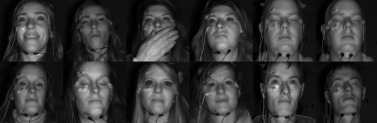
\includegraphics[scale=1]{gambar/3_1_5.jpg}
  % Keterangan gambar yang diinputkan
  \caption{Dataset DROZY}
  % Label referensi dari gambar yang diinputkan
  \label{fig:Drozy}
\end{figure}


\subsection{Dataset UTA-RLDD}
\label{subsec:UTARLDD}

Dataset RLDD terdiri dari sekitar 30 jam video RGB dari 50 partisipan yang sehat. Untuk setiap partisipan, kami memperoleh satu video untuk masing-masing dari tiga kelas yang berbeda: kewaspadaan, kewaspadaan rendah, dan kantuk, dengan total 50 video. Subjek penelitian adalah mahasiswa sarjana atau pascasarjana dan anggota staf yang berpartisipasi secara sukarela atau setelah menerima kredit tambahan dalam sebuah kursus. Semua partisipan berusia di atas 18 tahun.
Video diambil dari berbagai sudut yang berbeda di lingkungan dan latar belakang kehidupan nyata. Setiap video direkam sendiri oleh partisipan, menggunakan ponsel atau kamera web mereka. Kecepatan frame selalu kurang dari 30 fps, yang merupakan kecepatan frame yang diharapkan dari kamera tipikal yang digunakan oleh masyarakat umum.

\begin{figure} [H] \centering
  % Nama dari file gambar yang diinputkan
  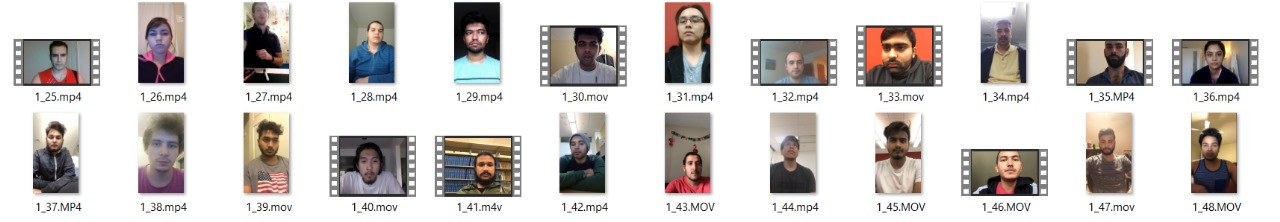
\includegraphics[width=\textwidth]{gambar/uta.jpg}
  % Keterangan gambar yang diinputkan
  \caption{Dataset UTA-RLDD}
  % Label referensi dari gambar yang diinputkan
  \label{fig:UTARLDD}
\end{figure}


\subsection{Peralatan dan Perangkat}
Pada Penelitian ini digunakan perangkat laptop dengan spesifikasi RAM 16 GB, Processor AMD Ryzen 5 4600H, graphic card NVIDIA GeForce GTX 1650, selain itu untuk melakukan training model dan lain lain digunakan Kaggle dan PyCharm. PyCharm adalah Integrated Development Environment (IDE) yang digunakan untuk pemrograman Python. Kaggle digunakan untuk meningkatkan keterampilan data untuk mendapatkan model, sedangkan PyCharm digunakan untuk Preprocessing data video yang akan digunakan.

\cleardoublepage

% Bab 4 pengujian dan analisis
\chapter{HASIL DAN ANALISIS}
\label{chap:pengujiananalisis}

% Ubah bagian-bagian berikut dengan isi dari pengujian dan analisis

Pada penelitian ini dipaparkan mengenai pengujian dari model yang dibuat pada metodologi sebelumnya. Hasil pengujian kemudian akan dianalisis dan diharapkan dari hasil analisis didapatkan kesimpulan mengenai model yang dibuat dengan metode yang telah ditentukan.

\section{Hasil Pengumpulan Dataset}
\label{sec:HasilPengumpulanDataset}
Dengan Menggunakan dataset yang dimiliki dengan total video sebanyak 36 video untuk dataset DROZY dan 36 video untuk dataset UTA-RLDD. Kemudian berdasarkan nilai KSS yang dimiliki tiap dataset, video dikelompokkan berdasarkan kelas yang telah ditentukan. Pada penelitian ini digunakan 3 kelas klasifikasi yaitu Fokus sebagai kelas 1, kemudian waspada sebagai kelas 2, dan mengantuk sebagai kelas 3. Setelah dilakukan pengelompokan maka didapatkan jumlah video tiap kelas nya sebanyak 72 video seperti pada tabel berikut :

\begin{longtable}{|c|c|}
  \caption{Hasil Pengumpulan Video Dataset DROZY}
  \label{tb:HasilDrozy}                                   \\
  \hline
  \rowcolor[HTML]{C0C0C0}
  \textbf{Kelas} & \textbf{Total Video} \\
  \hline
  1            & 11  \\              
  2            & 10  \\              
  3            & 15  \\                           
  \hline
\end{longtable}


\begin{longtable}{|c|c|}
  \caption{Hasil Pengumpulan Video Dataset UTA-RLDD}
  \label{tb:HasilUTA}                                   \\
  \hline
  \rowcolor[HTML]{C0C0C0}
  \textbf{Kelas} & \textbf{Total Video} \\
  \hline
  1            & 12  \\              
  2            & 12  \\              
  3            & 12  \\                           
  \hline
\end{longtable}

\section{Hasil Ekstraksi Openness dan MAR}
\label{sec:skenariopengujian}
Kemudian dengan menggunakan video yang telah disaring sebagai dataset, maka dilakukan ekstraksi nilai PERCLOS dan MAR secara bersamaan. Pada penelitian ini digunakan DLib sebagai library untuk mengekstrak fitur mata dan mulut untuk kemudian dicari nilai PERCLOS dan MAR nya. Untuk MAR sendiri, prinsip yang digunakan untuk mendapatkan nilai MAR nya adalah sama dengan menggunakan rumus yang ada pada rumus 2.2. Sedangkan untuk mendapatkan nilai perclos, digunakan metode grayscaling untuk mengubah bagian mata menjadi hitam dan putih dimana selanjutnya bagian tersebut diubah menjadi nilai binary yang kemudian digunakan untuk menghitung nilai PERCLOS. Sehingga pada saat video dataset digunakan dan diekstraksi, didapatkan hasil seperti pada tabel berikut :

\begin{longtable}{|c|c|c|}
  \caption{Hasil Ekstraksi Openness dan MAR}
  \label{tb:openessMar}                                   \\
  \hline
  \rowcolor[HTML]{C0C0C0}
  \textbf{Frame} & \textbf{Openness} & \textbf{MAR\_Std} \\
  \hline
  1     & 0.33275762637414663 & 0.38539513718352214 \\
2     & 0.34874697414643113 & 0.4205568267370099  \\
3     & 0.360703620018165   & 0.40674460840998033 \\
4     & 0.3507866493276178  & 0.4029997011463999  \\
5     & 0.37454249196259926 & 0.4044786041022079  \\
6     & 0.3634563454911023  & 0.4044786041022079  \\
7     & 0.3321819194149599  & 0.3992242079377172  \\
8     & 0.3504649829636901  & 0.3992242079377172  \\
9     & 0.35549913081642326 & 0.4205568267370099  \\
10    & 0.3321819194149599  & 0.38539513718352214 \\
11    & 0.39724856953743126 & 0.441461136857296   \\
12    & 0.396521810060564   & 0.4817688377401808  \\
13    & 0.37037209526233333 & 0.42857142857142855 \\
14    & 0.39879948581769054 & 0.43103448275862066 \\
15    & 0.3049122660070178  & 0.5163798686058965  \\
16    & 0.36913816367292046 & 0.4483684122840496  \\
17    & 0.339167882784403   & 0.46524072383701487 \\
18    & 0.33473776085298823 & 0.5163798686058965  \\
19    & 0.35250465814487686 & 0.5010276520641941  \\
20    & 0.3119962564107116  & 0.5158420163115394  \\
21    & 0.30794387116508537 & 0.48392930804193357 \\
22    & 0.3091464381584206  & 0.5322912490583706  \\
23    & 0.31764220460752973 & 0.48392930804193357 \\
24    & 0.34089299776947407 & 0.516700085132471   \\
25    & 0.33275762637414663 & 0.4669998667732268  \\
26    & 0.35557477709288077 & 0.4500832232901259  \\
27    & 0.33275762637414663 & 0.4824718617569043  \\
28    & 0.3199371135536338  & 0.4703399055538226  \\
29    & 0.31455209784873994 & 0.5166666666666667  \\
30    & 0.3510495490185498  & 0.46880512375776673 \\
..... & ..... & ..... \\
17863 & 0.3713578569993685  & 0.4596324410120231  \\
17864 & 0.35557477709288077 & 0.41682550409799923 \\

  \hline
\end{longtable}

\section{Hasil Interpolasi Openness dan MAR}
\label{sec:Interpolasihasil}

Kemudian pada saat ekstraksi, ditemukan adanya frame yang tidak terdeteksi facial landmarknya sehingga menyebabkan nilai Openness dan MAR nya menjadi 0. Oleh karena itu dilakukan rekonstruksi atau perbaikan nilai sintesis dengan metode interpolasi. Metode interpolasi yang digunakan disini ialah metode interpolasi linear. Metode ini bisa membuat data sintesis baru dengan memperhatikan data data yang didapatkan sebelumnya. Dengan menggunakan perhitungan tertentu, interpolasi linear membentuk kembali data yang dianggap hilang karena facial landmarksnya tidak terdeteksi. hasilnya dapat dilihat pada tabel.

\begin{longtable}{|c|c|c|}
  \caption{Hasil sebelum Interpolasi}
  \label{tb:InterpolasiHasil}                                   \\
  \hline
  \rowcolor[HTML]{C0C0C0}
  \textbf{Frame} & \textbf{Openness} & \textbf{MAR\_Std} \\
  \hline
  14991 & 0.375743785003394 & 0.40920672838862215 \\
  14992 & 0.375743785003394 & 0.40920672838862215 \\
  14993 & 0 & 0 \\
  14994 & 0 & 0 \\
  14995 & 0.29900542119735485 & 0.4447896239237299 \\
  14996 & 0.29900542119735485 & 0.4447896239237299 \\
  14997 & 0.3134717215453426 & 0.4415485454008298 \\
  14998 & 0.3134717215453426 & 0.4415485454008298 \\
  14999 & 0.3237609520325029 & 0.447213595499958 \\
  15000 & 0.34624551912778445 & 0.4382053157856714 \\
  15001 & 0 & 0 \\
  15002 & 0 & 0 \\
  15003 & 0.26251162333210865 & 0.44409276770884176 \\
  15004 & 0.26251162333210865 & 0.44409276770884176 \\
  15005 & 0.32489118787869253 & 0.4473310158641847 \\
  \hline
\end{longtable}

\begin{longtable}{|c|c|c|}
  \caption{Hasil sesudah Interpolasi}
  \label{tb:InterpolasiHasil}                                   \\
  \hline
  \rowcolor[HTML]{C0C0C0}
  \textbf{Frame} & \textbf{Openness} & \textbf{MAR\_Std} \\
  \hline
  14991 & 0.375743785003394 & 0.40920672838862215 \\
  14992 & 0.375743785003394 & 0.40920672838862215 \\
  14993 & 0.35016433040138095 & 0.42106769356699136 \\
  14994 & 0.32458487579936784 & 0.43292865874536063 \\
  14995 & 0.29900542119735485 & 0.4447896239237299 \\
  14996 & 0.29900542119735485 & 0.4447896239237299 \\
  14997 & 0.3134717215453426 & 0.4415485454008298 \\
  14998 & 0.3134717215453426 & 0.4415485454008298 \\
  14999 & 0.3237609520325029 & 0.447213595499958 \\
  15000 & 0.34624551912778445 & 0.4382053157856714 \\
  15001 & 0.3183342205292258 & 0.4401677997600615 \\
  15002 & 0.2904229219306672 & 0.4421302837344516 \\
  15003 & 0.26251162333210865 & 0.44409276770884176 \\
  15004 & 0.26251162333210865 & 0.44409276770884176 \\
  15005 & 0.32489118787869253 & 0.4473310158641847 \\
  \hline
\end{longtable}



\section{Hasil Ekstraksi PERCLOS dan MAR}
\label{sec:PERCLOSMAR}
Setelah didapatkan nilai bukaan mata dan mulut, selanjutnya dilakukan perhitungan lanjutan untuk mendapatkan nilai PERCLOS dan MAR. Untuk mendapatkan nilai perclos digunakan satu interval waktu yang sama yaitu 1 detik. Sehingga setiap 30 frame data Openess dan MAR akan menghasilkan satu data PERCLOS dan MAR. Data PERCLOS yang didapatkan berbeda beda jumlah nya karena total frame pada satu dataset berbeda beda. Sehingga pada saat video dataset diekstraksi nilai PERCLOSnya, didapatkan hasil seperti pada tabel berikut :

\begin{longtable}{|c|c|c|}
  \caption{Hasil Ekstraksi PERCLOS dan MAR}
  \label{tb:EnergiKecepatan}                                   \\
  \hline
  \rowcolor[HTML]{C0C0C0}
  \textbf{No} & \textbf{PERCLOS} & \textbf{MAR\_Std} \\
  \hline
  1     & 0.04341892752775   & 0.0246262117542063 \\
  2     & 0.0457977178822792 & 0.0286218820410614 \\
  3     & 0.0363179516630053 & 0.0193095358670792 \\
  4     & 0.0590892249621408 & 0.0192869144310238 \\
  5     & 0.040213924189683  & 0.0164477395589993 \\
  6     & 0.0604693124683611 & 0.0164027809907854 \\
  7     & 0.0418428937527917 & 0.0175763328675194 \\
  8     & 0.0367099233744161 & 0.0170944891422672 \\
  9     & 0.0460220195416752 & 0.0297215001851705 \\
  10    & 0.1058752799978109 & 0.0290507174502237 \\
  11    & 0.0762559420253322 & 0.0253128481686185 \\
  12    & 0.0273801000576773 & 0.0180387417110928 \\
  13    & 0.1081582077308788 & 0.01263547199005   \\
  14    & 0.0234176774284208 & 0.018918924189878  \\
  15    & 0.0268128099330071 & 0.0169950902266086 \\
  16    & 0.1166419802226671 & 0.0218784895345093 \\
  17    & 0.0269244763591171 & 0.0239784396847136 \\
  18    & 0.1742677324661242 & 0.0252603962094769 \\
  19    & 0.2223696034435887 & 0.0263079806866737 \\
  20    & 0.0560419283453739 & 0.021425279810804  \\
  21    & 0.0209232346119773 & 0.0276537569920319 \\
  22    & 0.1407170390627357 & 0.0142564138587645 \\
  23    & 0.1315659177009895 & 0.0303915062546408 \\
  24    & 0.1288284404723541 & 0.0283789867675656 \\
  25    & 0.0960669098066907 & 0.0169481889120284 \\
  26    & 0.0534638035142962 & 0.0188981368675101 \\
  27    & 0.1418466367232676 & 0.012678303659045  \\
  28    & 0.0514559005190815 & 0.0122696792726204 \\
  29    & 0.0811347901146985 & 0.0164486221578006 \\
  30    & 0.4143576236766674 & 0.025550198457152  \\
  31    & 0.4868099464310756 & 0.0245221496475319 \\
  32    & 0.1068540476432911 & 0.0299960526372281 \\
  33    & 0.0481730883150443 & 0.0195896829812593 \\
  34    & 0.0414214305253392 & 0.0201600340611569 \\
  ..... & .....              & .....              \\
  393   & 0.1099072500438651 & 0.0170603553394825 \\

  \hline
\end{longtable}


\section{Hasil Preprocessing}
\label{sec:skenariopengujian}

Kemudian setelah nilai PERCLOS dan MAR nya berhasil didapatkan dari semua video dataset yang dimiliki, selanjutnya data tersebut dilanjutkan untuk masuk ke proses preprosesing. Pada tahap ini data data yang dimiliki akan dirapihkan dan kemudian dilakukan tahap tahap tertentu untuk menghasilkan data yang baik dimana data tersebut nantinya akan digunakan untuk proses training yang akan menciptakan model klasifikasi yang diharapkan.

\subsection{Balancing data}
Proses ini bertujuan untuk menyamakan jumlah data yang akan digunakan pada satu csv sebagai data. Penyamaan data digunakan dengan mengambil jumlah data paling sedikit sebagai acuan. Kemudian, didapatkan data paling sedikit yaitu sebanyak 112 data PERCLOS. Sehingga, untuk setiap CSV lainnya dilakukan pemotongan dengan mengambil 56 data awal dan 56 data akhir. Dapat dilihat pada tabel berikut.

\begin{longtable}{|c|c|c|}
  \caption{Data sebelum Pemotongan}
  \label{tb:sebelumpemotongan}                                   \\
  \hline
  \rowcolor[HTML]{C0C0C0}
  \textbf{Frame} & \textbf{PERCLOS} & \textbf{MAR} \\
  \hline
  1   & 0.1816528805118815 & 0.0173268322049449 \\
  2   & 0.0813165253840059 & 0.0202092879889068 \\
  3   & 0.1120012122388704 & 0.0236920685734675 \\
  4   & 0.0266037854461568 & 0.0119342103718461 \\
  5   & 0.0548462886307339 & 0.0235971937432285 \\
  6   & 0.0274694311138857 & 0.0161956019049888 \\
  7   & 0.0230377767734855 & 0.0195442314445453 \\
  8   & 0.0855786310601608 & 0.0191941177515545 \\
  9   & 0.1073765364498199 & 0.0146704493597198 \\
  10  & 0.1279653706800781 & 0.0209992139810568 \\
  11  & 0.028553141344168  & 0.0155181204012414 \\
  12  & 0.0293475318026248 & 0.0171695763546431 \\
  13  & 0.0290516626494758 & 0.0175816675234297 \\
  14  & 0.0776266967312657 & 0.0162103135247574 \\
  15  & 0.0281624221693752 & 0.0143011344691447 \\
  16  & 0.0553772215885699 & 0.0189356774322395 \\
  17  & 0.0266618970156669 & 0.0234303973615371 \\
  18  & 0.1107976881202639 & 0.0148835680324435 \\
  19  & 0.0247546442197618 & 0.0155388337888783 \\
  20  & 0.1078013876301218 & 0.0143790040239863 \\
  21  & 0.0286570283892652 & 0.0223078445947027 \\
  22  & 0.0261035183669317 & 0.0196738367551345 \\
  23  & 0.0546274615438689 & 0.0166035900394699 \\
  24  & 0.0272482250599491 & 0.0145434570859087 \\
  25  & 0.0254242296155474 & 0.0175244013838591 \\
  26  & 0.0293822224756522 & 0.0132305209721131 \\
  27  & 0.0806260483855669 & 0.0193947087641066 \\
  28  & 0.0274583434798892 & 0.0171066269402163 \\
  29  & 0.0255342443673257 & 0.0174210466661458 \\
  30  & 0.0544727255873108 & 0.0109366040975671 \\
  31  & 0.3739304556338749 & 0.0139806642241198 \\
  ..... & ..... & ..... \\
  249 & 0.2223552668712169 & 0.0182882169245095 \\

  \hline
\end{longtable}

\begin{longtable}{|c|c|c|}
  \caption{Data setelah Pemotongan}
  \label{tb:setelahPemotongan}                                   \\
  \hline
  \rowcolor[HTML]{C0C0C0}
  \textbf{Frame} & \textbf{PERCLOS} & \textbf{MAR} \\
  \hline
  1   & 0.1816528805118815 & 0.0173268322049449 \\
  2   & 0.0813165253840059 & 0.0202092879889068 \\
  3   & 0.1120012122388704 & 0.0236920685734675 \\
  4   & 0.0266037854461568 & 0.0119342103718461 \\
  5   & 0.0548462886307339 & 0.0235971937432285 \\
  6   & 0.0274694311138857 & 0.0161956019049888 \\
  7   & 0.0230377767734855 & 0.0195442314445453 \\
  8   & 0.0855786310601608 & 0.0191941177515545 \\
  9   & 0.1073765364498199 & 0.0146704493597198 \\
  10  & 0.1279653706800781 & 0.0209992139810568 \\
  11  & 0.028553141344168  & 0.0155181204012414 \\
  12  & 0.0293475318026248 & 0.0171695763546431 \\
  13  & 0.0290516626494758 & 0.0175816675234297 \\
  14  & 0.0776266967312657 & 0.0162103135247574 \\
  15  & 0.0281624221693752 & 0.0143011344691447 \\
  16  & 0.0553772215885699 & 0.0189356774322395 \\
  17  & 0.0266618970156669 & 0.0234303973615371 \\
  18  & 0.1107976881202639 & 0.0148835680324435 \\
  19  & 0.0247546442197618 & 0.0155388337888783 \\
  20  & 0.1078013876301218 & 0.0143790040239863 \\
  21  & 0.0286570283892652 & 0.0223078445947027 \\
  22  & 0.0261035183669317 & 0.0196738367551345 \\
  23  & 0.0546274615438689 & 0.0166035900394699 \\
  24  & 0.0272482250599491 & 0.0145434570859087 \\
  25  & 0.0254242296155474 & 0.0175244013838591 \\
  26  & 0.0293822224756522 & 0.0132305209721131 \\
  27  & 0.0806260483855669 & 0.0193947087641066 \\
  28  & 0.0274583434798892 & 0.0171066269402163 \\
  29  & 0.0255342443673257 & 0.0174210466661458 \\
  30  & 0.0544727255873108 & 0.0109366040975671 \\
  31  & 0.3739304556338749 & 0.0139806642241198 \\
  ..... & ..... & ..... \\
  112 & 0.1015446046460651 & 0.0170760931016739 \\
  \hline
\end{longtable}

\subsection{Hasil Labeling}
Pada tahap ini, setiap dataset yang dimiliki dari video yang digunakan akan diberikan label berdasarkan nilai KSS yang telah didapatkan dan kemudian dimasukkan kedalam kelas yang telah ditentukan sesuai dengan pembagian kelas tingkat kantuk skala karolinska. Proses dimulai dengan menambahkan kolom baru kedalam file csv yang dimiliki, dimana kolom ini digunakan sebagai identitas kelas sebagai label oleh data yang dimiliki. Berikut merupakan hasil labeling pada dataset yang dimiliki.


\begin{longtable}{|c|c|c|}
  \caption{Data sebelum Labeling}
  \label{tb:DatasebelumLabel}                                   \\
  \hline
  \rowcolor[HTML]{C0C0C0}
  \textbf{Frame} & \textbf{PERCLOS} & \textbf{MAR} \\
  \hline


  1 & 0.0379261534386973 & 0.0252017735374091 \\
  2 & 0.0298956056778338 & 0.0214426506252242 \\
  3 & 0.0322315266828644 & 0.0221272159006492 \\
  4 & 0.0317349009938341 & 0.0169105984899276 \\
  5 & 0.0448629264100697 & 0.0166322852613973 \\
  6 & 0.0398516212423454 & 0.0110885559580576 \\
  7 & 0.0376917358534904 & 0.0143518814787156 \\
  8 & 0.0321941677552277 & 0.0161108532000975 \\
  9 & 0.0347334084658292 & 0.0177275899053815 \\
  10 & 0.0294942344020012 & 0.0308730659997332 \\
  11 & 0.023949691261859  & 0.0295632878714494 \\
  12 & 0.0856134255183379 & 0.0380256171355866 \\
  13 & 0.0323445445990112 & 0.0195737989150442 \\
  14 & 0.2117050730658914 & 0.028119378775709  \\
  15 & 0.038876268851734  & 0.0155395239368325 \\
  16 & 0.0265444419381986 & 0.0191109930279671 \\
  17 & 0.0284200639510221 & 0.0243439023319811 \\
  18 & 0.1005344404888114 & 0.0281761938359568 \\
  19 & 0.0286532003172247 & 0.0205196259227119 \\
  20 & 0.0297490481675679 & 0.0305405474736834 \\
  21 & 0.0276267827433371 & 0.0236279809099732 \\
  22 & 0.0616410693009279 & 0.0387297862508864 \\
  23 & 0.2117084736442856 & 0.0530036875401317 \\
  24 & 0.1234691311855758 & 0.0162842335613543 \\
  25 & 0.0140914643859832 & 0.0157622505798132 \\
  26 & 0.0885215166889441 & 0.0243724463064474 \\
  27 & 0.2786408347943638 & 0.0149082820223585 \\
  ..... & ..... & ..... \\
  112 & 0.4583778787184472 & 0.0145344028391528 \\

  \hline
\end{longtable}

\begin{longtable}{|c|c|c|c|}
  \caption{Data sesudah Labeling}
  \label{tb:DatasesudahLabel}                                   \\
  \hline
  \rowcolor[HTML]{C0C0C0}
  \textbf{Frame} & \textbf{PERCLOS} & \textbf{MAR} & \textbf{Kelas} \\
  \hline
  1 & 0.0379261534386973 & 0.0252017735374091 & 1 \\
  2 & 0.0298956056778338 & 0.0214426506252242 & 1 \\
  3 & 0.0322315266828644 & 0.0221272159006492 & 1\\
  4 & 0.0317349009938341 & 0.0169105984899276  & 1\\
  5 & 0.0448629264100697 & 0.0166322852613973 & 1 \\
  6 & 0.0398516212423454 & 0.0110885559580576 & 1 \\
  7 & 0.0376917358534904 & 0.0143518814787156 & 1 \\
  8 & 0.0321941677552277 & 0.0161108532000975 & 1 \\
  9 & 0.0347334084658292 & 0.0177275899053815 & 1 \\
  10 & 0.0294942344020012 & 0.0308730659997332 & 1 \\
  11 & 0.023949691261859  & 0.0295632878714494 & 1 \\
  12 & 0.0856134255183379 & 0.0380256171355866 & 1 \\
  13 & 0.0323445445990112 & 0.0195737989150442 & 1 \\
  14 & 0.2117050730658914 & 0.028119378775709 & 1  \\
  15 & 0.038876268851734  & 0.0155395239368325 & 1 \\
  16 & 0.0265444419381986 & 0.0191109930279671 & 1 \\
  17 & 0.0284200639510221 & 0.0243439023319811 & 1 \\
  18 & 0.1005344404888114 & 0.0281761938359568 & 1 \\
  19 & 0.0286532003172247 & 0.0205196259227119 & 1 \\
  20 & 0.0297490481675679 & 0.0305405474736834 & 1 \\
  21 & 0.0276267827433371 & 0.0236279809099732 & 1 \\
  22 & 0.0616410693009279 & 0.0387297862508864 & 1 \\
  23 & 0.2117084736442856 & 0.0530036875401317 & 1 \\
  24 & 0.1234691311855758 & 0.0162842335613543 & 1 \\
  25 & 0.0140914643859832 & 0.0157622505798132 & 1 \\
  26 & 0.0885215166889441 & 0.0243724463064474 & 1 \\
  27 & 0.2786408347943638 & 0.0149082820223585 & 1 \\
  ..... & ..... & ..... & 1\\
  112 & 0.4583778787184472 & 0.0145344028391528 & 1 \\
  \hline
\end{longtable}

Proses yang sama juga dilakukan untuk setiap file csv yang dimiliki sehingga dapat dilihat pada tabel berikut ini. Setelah dilakukan labeling terhadap semua dataset yang dimiliki, selanjutnya dilakukan penggabungan data menjadi satu file.

\begin{longtable}{|c|c|c|}
  \caption{Hasil Label pada setiap data}
  \label{tb:HasilEkstraksiPERCLOS}                                   \\
  \hline
  \rowcolor[HTML]{C0C0C0}
  \textbf{Video} & \textbf{Total Frame} & \textbf{Kelas} \\
  \hline
  1-1  & 17865 & 1     \\ 
  1-2 & 18994   & 2 \\ 
  1-3 & 17732  & 3 \\ 
  10-1  & 17866 & 1 \\ 
  10-3 & 17889 & 3 \\ 
  11-1 & 17914 & 3 \\ 
  11-2  & 17886 & 2 \\  
  11-3 & 17875 & 3 \\
  12-1 & 17889 & 1 \\
  13-1  & 17902 & 1 \\
  13-2 & 17900 & 2 \\
  14-1 & 17883  & 3 \\
  14-2  & 17861 & 2 \\
  14-3 & 17918  & 3 \\
  2-1 & 17899  & 1 \\
  2-2  & 18802  & 2 \\
  2-3 & 16292  & 3 \\
  3-1 & 17882 & 1 \\
  3-2  & 17696 & 1 \\
  3-3 & 17748 & 2 \\
  4-1 & 17789 & 3 \\
  4-2  & 16926 & 2 \\
  4-3 & 17791 & 3 \\
  5-1 & 17919  & 1 \\
  5-2  & 16350 & 3 \\
  5-3 & 16460 & 3 \\
  6-1 & 17913 & 1 \\
  6-2 & 17704 & 1 \\
  6-3  & 17914  & 3 \\
  7-2 & 15824 & 2 \\
  7-3 & 17756  & 3 \\
  8-1 & 17863  & 1 \\
  8-2  & 17748  & 2 \\
  8-3 & 18050 & 3 \\
  9-2 & 17908 & 2 \\
  9-3  & 17922  & 3 \\
  \hline
\end{longtable}

\subsection{Hasil Balancing}
Dalam tahap ini, akan diuraikan proses penyeimbangan data. Karena adanya variasi distribusi kelas yang asli dalam dataset, sangat penting untuk menyesuaikan proporsi ini untuk mencegah bias pada model terhadap kelas yang lebih sering muncul. Penyeimbangan ini dilakukan dengan cara menambahkan jumlah pada kelas yang kurang terwakili atau mengurangi jumlah pada kelas yang terlalu dominan, sehingga memastikan distribusi yang lebih merata di seluruh kategori. Langkah ini krusial karena memiliki pengaruh langsung terhadap efektivitas dan keseimbangan model klasifikasi. Penyesuaian yang dilakukan memastikan bahwa setiap kelas memiliki kontribusi yang seimbang dalam pelatihan model, yang pada akhirnya meningkatkan akurasi dan keandalan model dalam menghadapi data baru yang belum pernah dilihat sebelumnya. Dapat dilihat data sebelum adanya balancing pada tabel berikut :


\begin{longtable}{|c|c|}
  \caption{Sebaran Kelas sebelum Balancing}
  \label{tb:SebaranKelasbf}                                   \\
  \hline
  \rowcolor[HTML]{C0C0C0}
 \textbf{Kelas} & \textbf{Total Frame} \\
  \hline
 1 & 11 \\
  2 & 10 \\
 3 & 15 \\
  \hline
\end{longtable}

\begin{longtable}{|c|c|}
  \caption{Sebaran Kelas sesudah Balancing}
  \label{tb:EnergiKecepatan}                                   \\
  \hline
  \rowcolor[HTML]{C0C0C0}
 \textbf{Kelas} & \textbf{Total Frame} \\
  \hline
 1 & 35 \\
  2 & 35 \\
 3 & 35 \\
  \hline
\end{longtable}


\subsection{Hasil Standarisasi}
Setelah proses penyeimbangan data selesai, langkah selanjutnya adalah standarisasi data, yang bertujuan untuk membawa semua fitur ke skala yang sama. Hal ini penting karena fitur dengan rentang nilai yang lebih besar dapat mendominasi cara model mempelajari data, yang bisa berakibat buruk pada performa model. Dalam standarisasi, setiap fitur di dataset dikurangi dengan rata-rata (mean) dan dibagi dengan standar deviasi dari fitur tersebut. Proses ini menghasilkan fitur dengan rata-rata nol dan variansi satu, sehingga semua fitur memiliki pengaruh yang serupa saat proses pelatihan model.

Proses standarisasi ini tidak hanya memudahkan proses pelatihan tetapi juga membantu dalam mengurangi kemungkinan overfitting, karena model tidak lagi sensitif terhadap skala dari input fitur. Seperti terlihat pada Tabel 4.14 dan 4.15, nilai X telah diubah setelah standarisasi, memastikan bahwa penyeimbangan yang telah dilakukan tidak dipengaruhi oleh skala nilai yang tidak konsisten antar fitur.

\begin{longtable}{|c|c|}
  \caption{Data sebelum Standarisasi}
  \label{tb:bfStandard}                                   \\
  \hline
  \rowcolor[HTML]{C0C0C0}
  \textbf{X} & \textbf{Y} \\
  \hline
  {[}0.04341893 0.04579772 0.03631795 ... 0.02739552 0.02141735 0.02616562{]} & 1  \\
  {[}0.04007385 0.09729903 0.05479942 ... 0.01899503 0.01977246 0.01517022{]} & 2  \\
  {[}0.04124125 0.0362592  0.05022096 ... 0.01572837 0.0138987  0.01706036{]} & 3  \\
  ..... & .....  \\
  {[}0.03226756 0.03462665 0.03260762 ... 0.01570125 0.01376602 0.01347413{]} & 3  \\
  {[}0.01630081 0.1169725  0.0295373  ... 0.02005795 0.0133355  0.01780213 {]} & 2  \\
  {[}0.02111398 0.08720713 0.11864278 ... 0.01903442 0.01896476 0.01991052{]} & 3\\
  \hline
\end{longtable}

\begin{longtable}{|c|c|}
  \caption{Data sesudah Standarisasi}
  \label{tb:afStandard}                                   \\
  \hline
  \rowcolor[HTML]{C0C0C0}
  \textbf{X} & \textbf{Y} \\
  \hline
  {[}0.02252558 0.15894138 0.02282446 ... 0.01349007 0.01333916 0.01389683{]} & 1  \\
  {[}0.04284438 0.08818944 0.08365624 ... 0.01365269 0.01408636 0.00171242{]} & 2  \\
  {[}0.05197581 0.04477653 0.0486499  ... 0.01924756 0.01689856 0.01649089{]} & 3  \\
  ..... & .....  \\
  {[}0.06360157 0.0395955  0.06357524 ... 0.01439066 0.01945191 0.01769325{]} & 3  \\
  {[}0.04007385 0.09729903 0.05479942 ... 0.01899503 0.01977246 0.01517022{]} & 2  \\
  {[}0.08423872 0.04564282 0.04092245 ... 0.01373789 0.01567853 0.01518549{]} & 3\\
  \hline
\end{longtable}

\section{Hasil Evaluasi Model}
\label{sec:HasilEvaluasiModel}

\subsection{SVM RBF Kernel}
\label{subsec:evalSVMRBF}

Pada gambar 4.1 ditampilkan confusion matrix dari hasil evaluasi model SVM dengan kernel RBF. Confusion matrix ini menunjukkan jumlah prediksi benar dan salah yang dibuat oleh model pada data uji. Terlihat bahwa model mampu memprediksi dengan benar 8 sampel kelas 1, 8 sampel kelas 2, dan 9 sampel kelas 3. Namun, terdapat beberapa kesalahan prediksi di mana 1 sampel kelas 1 diprediksi sebagai kelas 3, dan 1 sampel kelas 2 diprediksi sebagai kelas 3.

Visualisasi confusion matrix pada gambar 4.2 memperlihatkan distribusi prediksi model dengan lebih jelas. Warna yang lebih gelap menunjukkan jumlah prediksi yang lebih banyak, yang mengindikasikan bahwa sebagian besar sampel diuji telah diprediksi dengan benar oleh model.

Gambar 4.3 menampilkan laporan klasifikasi yang mencakup metrik-metrik evaluasi seperti precision, recall, f1-score, dan support untuk setiap kelas. Dari tabel ini dapat dilihat bahwa model memiliki precision sebesar 1.00 untuk kelas 1 dan kelas 2, serta 0.82 untuk kelas 3. Recall untuk kelas 1 dan kelas 2 adalah 0.89, sementara untuk kelas 3 adalah 1.00. Nilai f1-score menunjukkan keseimbangan antara precision dan recall, dengan nilai tertinggi pada kelas 1 dan kelas 2 (0.94) dan sedikit lebih rendah pada kelas 3 (0.90). Akurasi keseluruhan model adalah 0.93, yang berarti model mampu memprediksi dengan benar 93\% dari total sampel uji. Nilai rata-rata makro (macro avg) dan rata-rata berbobot (weighted avg) untuk precision, recall, dan f1-score juga menunjukkan performa model yang konsisten dan baik.

Secara keseluruhan, hasil evaluasi ini menunjukkan bahwa model SVM dengan kernel RBF memiliki kinerja yang sangat baik dalam mengklasifikasikan sampel-sampel pada data uji, dengan hanya sedikit kesalahan prediksi yang terjadi.

\begin{figure} [H] \centering
  % Nama dari file gambar yang diinputkan
  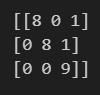
\includegraphics[scale=1]{gambar/cfrbf.jpg}
  % Keterangan gambar yang diinputkan
  \caption{Confusion Matrix SVM RBF Kernel}
  % Label referensi dari gambar yang diinputkan
  \label{fig:evalconfRBF}
\end{figure}

\begin{figure} [H] \centering
  % Nama dari file gambar yang diinputkan
  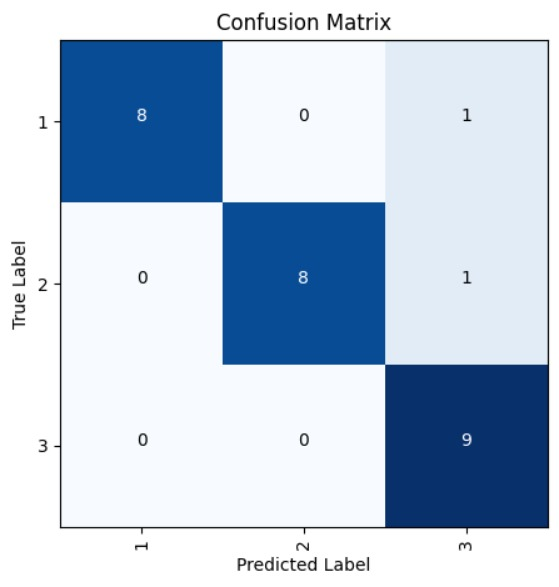
\includegraphics[scale=0.65]{gambar/cfprbf.jpg}
  % Keterangan gambar yang diinputkan
  \caption{visualisasi Confusion Matrix SVM RBF Kernel}
  % Label referensi dari gambar yang diinputkan
  \label{fig:evalconfpRBF}
\end{figure}


\begin{figure} [H] \centering
  % Nama dari file gambar yang diinputkan
  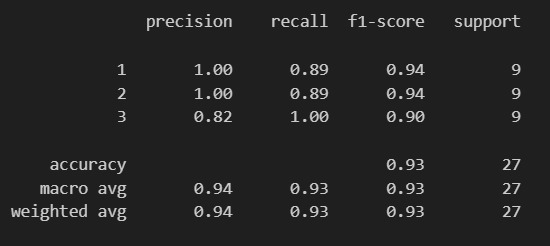
\includegraphics[scale=0.65]{gambar/evalrbf.jpg}
  % Keterangan gambar yang diinputkan
  \caption{Evaluasi SVM RBF Kernel}
  % Label referensi dari gambar yang diinputkan
  \label{fig:evalRBF}
\end{figure}

\subsection{SVM Linear Kernel}
\label{sec:evalLinearKernel}
Pada gambar 4.4 ditampilkan confusion matrix dari hasil evaluasi model SVM dengan kernel Linear. Confusion matrix ini menunjukkan jumlah prediksi benar dan salah yang dibuat oleh model pada data uji. Terlihat bahwa model mampu memprediksi dengan benar 8 sampel kelas 1, 8 sampel kelas 2, dan 9 sampel kelas 3. Namun, terdapat beberapa kesalahan prediksi di mana 1 sampel kelas 1 diprediksi sebagai kelas 3, dan 1 sampel kelas 2 diprediksi sebagai kelas 1.

Visualisasi confusion matrix pada gambar 4.5 memperlihatkan distribusi prediksi model dengan lebih jelas. Warna yang lebih gelap menunjukkan jumlah prediksi yang lebih banyak, yang mengindikasikan bahwa sebagian besar sampel diuji telah diprediksi dengan benar oleh model.

Gambar 4.6 menampilkan laporan klasifikasi yang mencakup metrik-metrik evaluasi seperti precision, recall, f1-score, dan support untuk setiap kelas. Dari tabel ini dapat dilihat bahwa model memiliki precision sebesar 0.89 untuk kelas 1, 0.89 untuk kelas 2, dan 1.00 untuk kelas 3. Recall untuk kelas 1 adalah 0.89, untuk kelas 2 adalah 0.89, dan untuk kelas 3 adalah 1.00. Nilai f1-score menunjukkan keseimbangan antara precision dan recall, dengan nilai tertinggi pada kelas 3 (0.95) dan sedikit lebih rendah pada kelas 1 dan kelas 2 (0.89). Akurasi keseluruhan model adalah 0.89, yang berarti model mampu memprediksi dengan benar 89\% dari total sampel uji. Nilai rata-rata makro (macro avg) dan rata-rata berbobot (weighted avg) untuk precision, recall, dan f1-score juga menunjukkan performa model yang cukup baik.

\begin{figure} [H] \centering
  % Nama dari file gambar yang diinputkan
  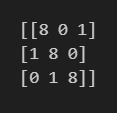
\includegraphics[scale=1]{gambar/cflinear.jpg}
  % Keterangan gambar yang diinputkan
  \caption{Confusion Matrix SVM Linear Kernel}
  % Label referensi dari gambar yang diinputkan
  \label{fig:evalconflinearkernel}
\end{figure}

\begin{figure} [H] \centering
  % Nama dari file gambar yang diinputkan
  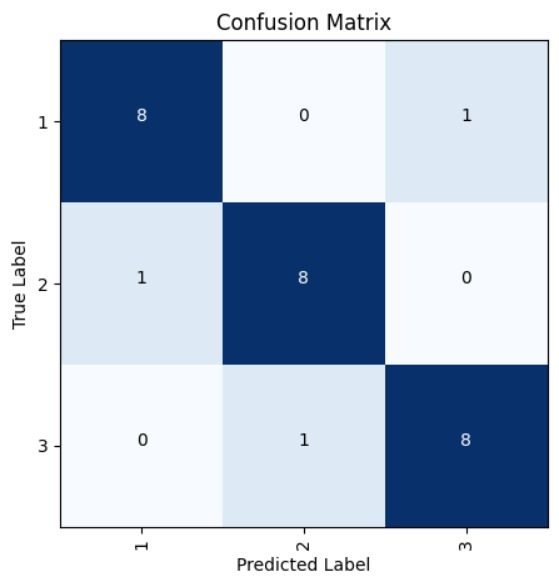
\includegraphics[scale=0.65]{gambar/cfplinear.jpg}
  % Keterangan gambar yang diinputkan
  \caption{Visualisasi Confusion Matrix SVM Linear Kernel}
  % Label referensi dari gambar yang diinputkan
  \label{fig:evalcfplinearkernel}
\end{figure}

\begin{figure} [H] \centering
  % Nama dari file gambar yang diinputkan
  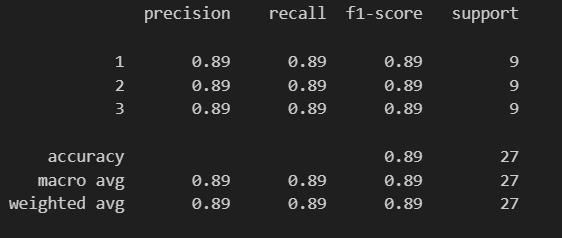
\includegraphics[scale=0.65]{gambar/EvalLinear.jpg}
  % Keterangan gambar yang diinputkan
  \caption{Evaluasi SVM Linear Kernel}
  % Label referensi dari gambar yang diinputkan
  \label{fig:evallinearkernel}
\end{figure}



\subsection{SVM Sigmoid Kernel}
\label{sec:evalSigmoidKernel}

Pada gambar 4.7 ditampilkan confusion matrix dari hasil evaluasi model SVM dengan kernel Sigmoid. Confusion matrix ini menunjukkan jumlah prediksi benar dan salah yang dibuat oleh model pada data uji. Terlihat bahwa model mampu memprediksi dengan benar 8 sampel kelas 1, 8 sampel kelas 2, dan 8 sampel kelas 3. Namun, terdapat beberapa kesalahan prediksi di mana 1 sampel kelas 1 diprediksi sebagai kelas 3, 1 sampel kelas 2 diprediksi sebagai kelas 1, dan 1 sampel kelas 3 diprediksi sebagai kelas 1.

Visualisasi confusion matrix pada gambar 4.8 memperlihatkan distribusi prediksi model dengan lebih jelas. Warna yang lebih gelap menunjukkan jumlah prediksi yang lebih banyak, yang mengindikasikan bahwa sebagian besar sampel diuji telah diprediksi dengan benar oleh model.

Gambar 4.9 menampilkan laporan klasifikasi yang mencakup metrik-metrik evaluasi seperti precision, recall, f1-score, dan support untuk setiap kelas. Dari tabel ini dapat dilihat bahwa model memiliki precision sebesar 0.89 untuk kelas 1, 1.00 untuk kelas 2, dan 0.89 untuk kelas 3. Recall untuk kelas 1 adalah 0.89, untuk kelas 2 adalah 0.89, dan untuk kelas 3 adalah 0.89. Nilai f1-score menunjukkan keseimbangan antara precision dan recall, dengan nilai tertinggi pada kelas 2 (0.94) dan sedikit lebih rendah pada kelas 1 dan kelas 3 (0.89). Akurasi keseluruhan model adalah 0.89, yang berarti model mampu memprediksi dengan benar 89\% dari total sampel uji. Nilai rata-rata makro (macro avg) dan rata-rata berbobot (weighted avg) untuk precision, recall, dan f1-score juga menunjukkan performa model yang cukup konsisten.

Secara keseluruhan, hasil evaluasi ini menunjukkan bahwa model SVM dengan kernel Sigmoid memiliki kemampuan yang baik dalam mengklasifikasikan sampel-sampel pada data uji, dengan beberapa kesalahan prediksi yang terjadi. Meskipun terdapat beberapa kesalahan dalam prediksi antar kelas, model ini masih menunjukkan tingkat akurasi yang tinggi dan dapat diandalkan untuk tugas klasifikasi pada dataset ini.

\begin{figure} [H] \centering
  % Nama dari file gambar yang diinputkan
  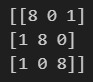
\includegraphics[scale=1]{gambar/cfsigmoid.jpg}
  % Keterangan gambar yang diinputkan
  \caption{Confusion Matrix SVM Sigmoid Kernel}
  % Label referensi dari gambar yang diinputkan
  \label{fig:evalcfsigmoidkernel}
\end{figure}

\begin{figure} [H] \centering
  % Nama dari file gambar yang diinputkan
  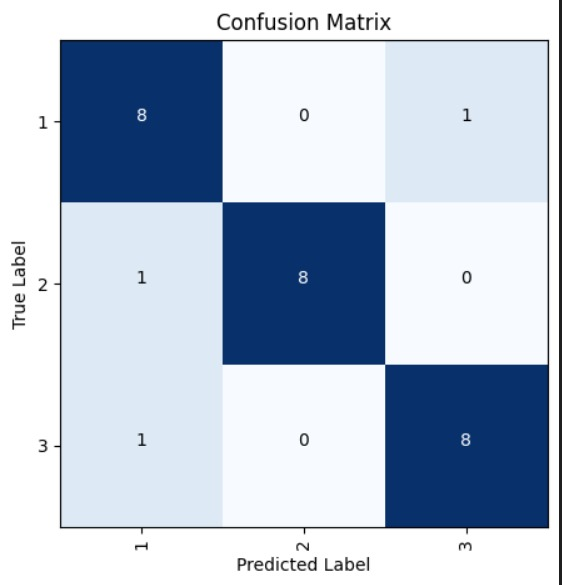
\includegraphics[scale=0.65]{gambar/cfpsigmoid.jpg}
  % Keterangan gambar yang diinputkan
  \caption{Visualisasi Confusion Matrix SVM Sigmoid Kernel}
  % Label referensi dari gambar yang diinputkan
  \label{fig:evalcfpsigmoidkernel}
\end{figure}

\begin{figure} [H] \centering
  % Nama dari file gambar yang diinputkan
  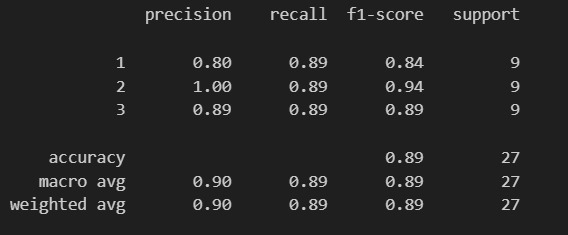
\includegraphics[scale=0.65]{gambar/evalsigmoid.jpg}
  % Keterangan gambar yang diinputkan
  \caption{Evaluasi SVM Sigmoid Kernel}
  % Label referensi dari gambar yang diinputkan
  \label{fig:evalsigmoidkernel}
\end{figure}


\subsection{SVM Polynomial Kernel}
\label{sec:evalPolyKernel}


Pada gambar 4.10 ditampilkan confusion matrix dari hasil evaluasi model SVM dengan kernel Polynomial. Confusion matrix ini menunjukkan jumlah prediksi benar dan salah yang dibuat oleh model pada data uji. Terlihat bahwa model mampu memprediksi dengan benar 9 sampel kelas 1, 8 sampel kelas 2, dan 7 sampel kelas 3. Namun, terdapat beberapa kesalahan prediksi di mana 1 sampel kelas 2 diprediksi sebagai kelas 1, dan 1 sampel kelas 3 diprediksi sebagai kelas 1.

Visualisasi confusion matrix pada gambar 4.11 memperlihatkan distribusi prediksi model dengan lebih jelas. Warna yang lebih gelap menunjukkan jumlah prediksi yang lebih banyak, yang mengindikasikan bahwa sebagian besar sampel diuji telah diprediksi dengan benar oleh model.

Gambar 4.12 menampilkan laporan klasifikasi yang mencakup metrik-metrik evaluasi seperti precision, recall, f1-score, dan support untuk setiap kelas. Dari tabel ini dapat dilihat bahwa model memiliki precision sebesar 0.82 untuk kelas 1, 0.89 untuk kelas 2, dan 1.00 untuk kelas 3. Recall untuk kelas 1 adalah 1.00, untuk kelas 2 adalah 0.89, dan untuk kelas 3 adalah 0.78. Nilai f1-score menunjukkan keseimbangan antara precision dan recall, dengan nilai tertinggi pada kelas 1 (0.90) dan sedikit lebih rendah pada kelas 2 (0.89) dan kelas 3 (0.88). Akurasi keseluruhan model adalah 0.89, yang berarti model mampu memprediksi dengan benar 89\% dari total sampel uji. Nilai rata-rata makro (macro avg) dan rata-rata berbobot (weighted avg) untuk precision, recall, dan f1-score juga menunjukkan performa model yang cukup baik.

\begin{figure} [H] \centering
  % Nama dari file gambar yang diinputkan
  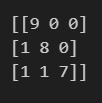
\includegraphics[scale=1]{gambar/cfpoly.jpg}
  % Keterangan gambar yang diinputkan
  \caption{Confusion Matrix SVM Polynomial Kernel}
  % Label referensi dari gambar yang diinputkan
  \label{fig:evalcfpolykernel}
\end{figure}

\begin{figure} [H] \centering
  % Nama dari file gambar yang diinputkan
  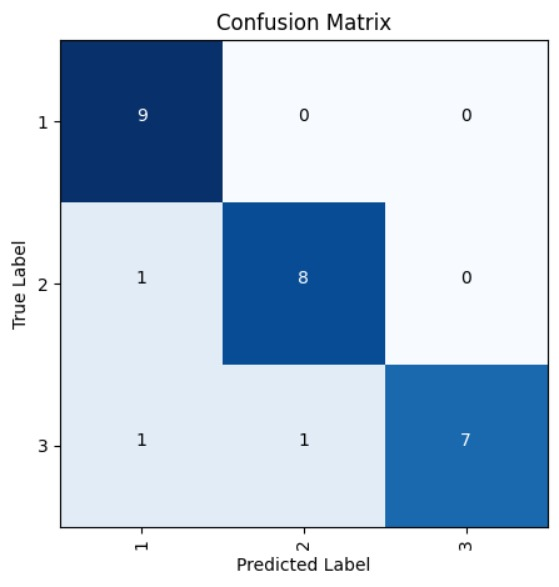
\includegraphics[scale=0.65]{gambar/cfppoly.jpg}
  % Keterangan gambar yang diinputkan
  \caption{Visualisasi Confusion Matrix SVM Polynomial Kernel}
  % Label referensi dari gambar yang diinputkan
  \label{fig:evalcfppolykernel}
\end{figure}

\begin{figure} [H] \centering
  % Nama dari file gambar yang diinputkan
  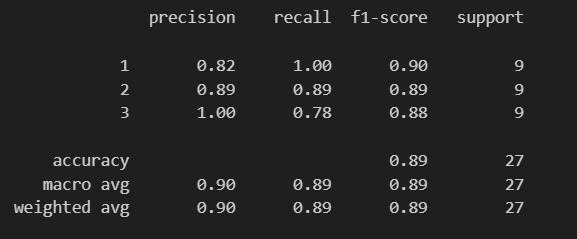
\includegraphics[scale=0.65]{gambar/evalpoly.jpg}
  % Keterangan gambar yang diinputkan
  \caption{Evakuasi SVM Polynomial Kernel}
  % Label referensi dari gambar yang diinputkan
  \label{fig:evalpolykernel}
\end{figure}

\subsection{Multi-Layer Perceptron (\emph{MLP})}
\label{sec:evalSigmoidKernel}

Pada gambar 4.13 ditampilkan confusion matrix dari hasil evaluasi model Multi-Layer Perceptron (MLP) selama proses training. Confusion matrix ini menunjukkan jumlah prediksi benar dan salah yang dibuat oleh model pada data uji. Terlihat bahwa model mampu memprediksi dengan benar 8 sampel kelas 1, 8 sampel kelas 2, dan 8 sampel kelas 3. Namun, terdapat beberapa kesalahan prediksi di mana 1 sampel kelas 1 diprediksi sebagai kelas 3, 1 sampel kelas 2 diprediksi sebagai kelas 1, dan 1 sampel kelas 3 diprediksi sebagai kelas 1.

Visualisasi confusion matrix pada gambar 4.14 memperlihatkan distribusi prediksi model dengan lebih jelas. Warna yang lebih gelap menunjukkan jumlah prediksi yang lebih banyak, yang mengindikasikan bahwa sebagian besar sampel diuji telah diprediksi dengan benar oleh model.

Gambar 4.15 menampilkan laporan klasifikasi yang mencakup metrik-metrik evaluasi seperti precision, recall, f1-score, dan support untuk setiap kelas. Dari tabel ini dapat dilihat bahwa model memiliki precision sebesar 0.80 untuk kelas 1, 1.00 untuk kelas 2, dan 0.89 untuk kelas 3. Recall untuk kelas 1 adalah 0.89, untuk kelas 2 adalah 0.89, dan untuk kelas 3 adalah 0.89. Nilai f1-score menunjukkan keseimbangan antara precision dan recall, dengan nilai tertinggi pada kelas 2 (0.94) dan sedikit lebih rendah pada kelas 1 (0.84) dan kelas 3 (0.89). Akurasi keseluruhan model adalah 0.89, yang berarti model mampu memprediksi dengan benar 89\% dari total sampel uji. Nilai rata-rata makro (macro avg) dan rata-rata berbobot (weighted avg) untuk precision, recall, dan f1-score juga menunjukkan performa model yang cukup konsisten.

Arsitektur model yang digunakan pada training ini adalah MLP dengan dua lapisan tersembunyi yang terdiri dari 5 dan 2 neuron masing-masing. Model dilatih menggunakan fungsi aktivasi ReLU (Rectified Linear Unit) dan solver Adam untuk optimasi. Jumlah iterasi maksimum yang digunakan adalah 100000, yang memastikan bahwa model mencapai konvergensi selama proses training. Akurasi model yang dicapai adalah 0.89, menunjukkan bahwa model ini memiliki kemampuan yang baik dalam mengklasifikasikan sampel-sampel pada data uji.

\begin{figure} [H] \centering
  % Nama dari file gambar yang diinputkan
  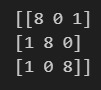
\includegraphics[scale=1]{gambar/cfmlp.jpg}
  % Keterangan gambar yang diinputkan
  \caption{Confusion Matrix MLP training}
  % Label referensi dari gambar yang diinputkan
  \label{fig:evalcfmlp}
\end{figure}

\begin{figure} [H] \centering
  % Nama dari file gambar yang diinputkan
  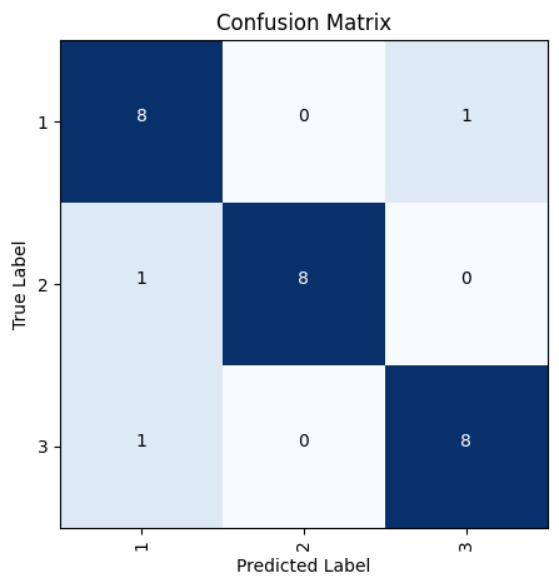
\includegraphics[scale=0.65]{gambar/cfpmlp.jpg}
  % Keterangan gambar yang diinputkan
  \caption{Visualisasi Confusion Matrix MLP training}
  % Label referensi dari gambar yang diinputkan
  \label{fig:evalcfpmlp}
\end{figure}

\begin{figure} [H] \centering
  % Nama dari file gambar yang diinputkan
  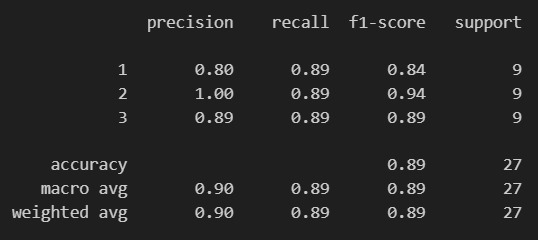
\includegraphics[scale=0.65]{gambar/evalmlp.jpg}
  % Keterangan gambar yang diinputkan
  \caption{Evaluasi Hasil training MLP}
  % Label referensi dari gambar yang diinputkan
  \label{fig:evalmlpl}
\end{figure}

\begin{figure} [H] \centering
  % Nama dari file gambar yang diinputkan
  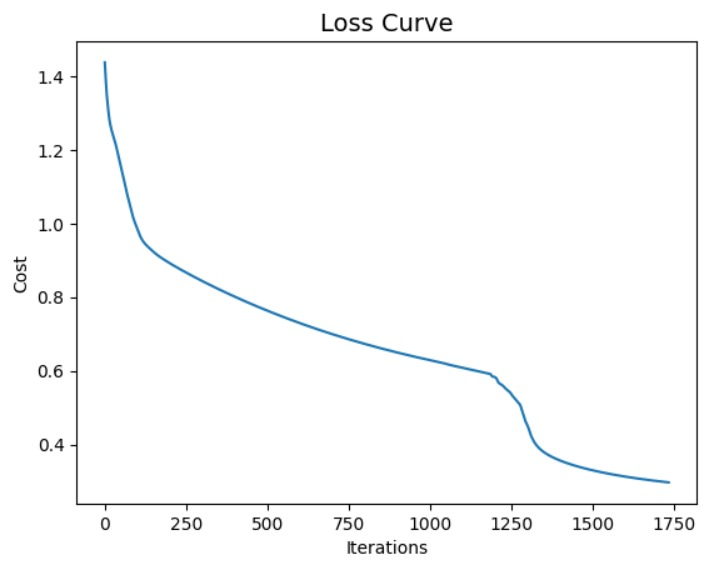
\includegraphics[scale=0.5]{gambar/lossmlp.jpg}
  % Keterangan gambar yang diinputkan
  \caption{Loss training MLP}
  % Label referensi dari gambar yang diinputkan
  \label{fig:lossmlp}
\end{figure}

\section{Hasil Pengujian Model}
\label{sec:skenariopengujian}
\begin{figure} [H] \centering
  % Nama dari file gambar yang diinputkan
  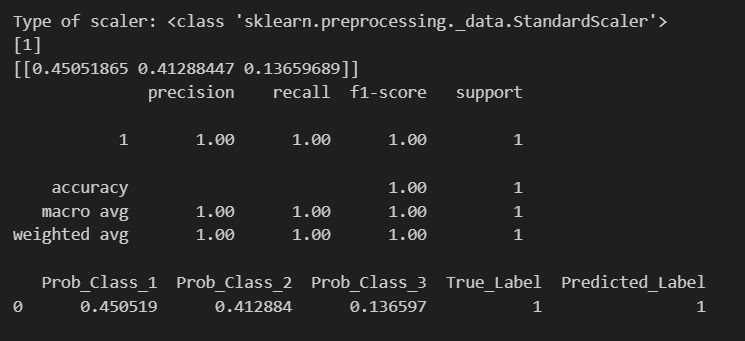
\includegraphics[scale=0.75]{gambar/predik.jpg}
  % Keterangan gambar yang diinputkan
  \caption{Hasil pengujian model}
  % Label referensi dari gambar yang diinputkan
  \label{fig:predikmodel}
\end{figure}


\section{Pembahasan}
\label{sec:skenariopengujian}


% \section{Evaluasi Pengujian}
% \label{sec:analisispengujian}

% Dari pengujian yang \lipsum[1]

% % Contoh pembuatan tabel

% \lipsum[2-4]

\cleardoublepage

% Bab 5 penutup
\chapter{PENUTUP}
\label{chap:penutup}

% Ubah bagian-bagian berikut dengan isi dari penutup

\section{Kesimpulan}
\label{sec:kesimpulan}

Berdasarkan hasil pengujian yang \lipsum[1][1-3] sebagai berikut:

\begin{enumerate}[nolistsep]

  \item Pembuatan \lipsum[2][1-3]

  \item \lipsum[2][4-6]

  \item \lipsum[2][7-10]

\end{enumerate}

\section{Saran}
\label{chap:saran}

Untuk pengembangan lebih lanjut pada \lipsum[1][1-3] antara lain:

\begin{enumerate}[nolistsep]

  \item Memperbaiki \lipsum[2][1-3]

  \item \lipsum[2][4-6]

  \item \lipsum[2][7-10]

\end{enumerate}

\cleardoublepage

\chapter*{DAFTAR PUSTAKA}
\addcontentsline{toc}{chapter}{DAFTAR PUSTAKA}
\renewcommand\refname{}
\vspace{2ex}
\renewcommand{\bibname}{}
\begingroup
\def\chapter*#1{}
\printbibliography
\endgroup
\cleardoublepage

% Biografi penulis
\begin{center}
  \Large
  \textbf{BIOGRAFI PENULIS}
\end{center}

\addcontentsline{toc}{chapter}{BIOGRAFI PENULIS}

\vspace{2ex}

\begin{wrapfigure}{L}{0.3\textwidth}
  \centering
  \vspace{-3ex}
  % Ubah file gambar berikut dengan file foto dari mahasiswa
  \includegraphics[width=0.3\textwidth]{gambar/joe.png}
  \vspace{-4ex}
\end{wrapfigure}

% Ubah kalimat berikut dengan biografi dari mahasiswa
\name{}, adalah penulis penelitian ini. Lahir dari Pasangan Bapak E. Napitupulu dan A. Manik dan merupakan anak ke 2 dari 3 bersaudara. Penulis lahir di Parapat tepatnya di Kabupaten Simalungun Sumatera Utara pada 08 November 2002. Penulis memulai pendidikan formal di SD Negeri N2091462 Parapat(2008-2014),SMP Negeri 1 Girsang Sipangan Bolon(2014-2017),SMA Swasta Rk. Bintang Timur Pematang Siantar(2017-2020). Kemudian setelah menyelesaikan pendidikan SMA di Pematang Siantar, Penulis melanjutkan studi S1 di Institut Teknologi Sepuluh Nopember di departemen Teknik Komputer. Penulis aktif berorganisasi di BEM Fakultas Teknologi Elektro dan Informatika Cerdas ITS(2022-2024) dan Juga merupakan anggota GenBI tahun 2022-2024. Penulis memiliki minat yang tinggi dibidang elektrikal dan dunia Internet Of Things(IoT). Pengalaman terakhirnya pada dibidang yang ditekuni yaitu internship atau magang selama 6 bulan di PT. Kalbe Farma Tbk, sebagai Industrial IoT and Automation Engineer.
\cleardoublepage

\end{document}
